\chapter{Data and Feature Research}
\label{ch:Data and Feature Research}

This chapter examines the empirical foundation and methodological framework underpinning the analysis of NIP in European investment-grade corporate bonds. The investigation progresses from data acquisition and preprocessing through feature selection and model development to performance validation. Initially, the chapter explores the extraction and refinement of bond data from Refinitiv, addressing challenges related to data quality and temporal bias. Subsequently, a structured approach for identifying and evaluating potential predictive features is developed based on economic rationale and statistical significance. The analysis then constructs a machine learning framework using XGBoost that transforms these features into actionable investment signals, with particular attention to optimizing the precision-recall tradeoff for maximum investment utility. The chapter concludes with a comprehensive backtest methodology that validates the model's efficacy under realistic market conditions. Throughout this analytical progression, the research maintains a consistent focus on translating complex statistical patterns into practical investment insights for fixed-income portfolio management.

\section{Data}
\label{sec:Data}

This study leverages comprehensive European corporate bond data extracted from the Refinitiv content layer API, which serves as the primary source for the training dataset employed in the machine learning algorithm. Refinitiv provides thorough coverage of fixed-income securities with detailed historical information, making it suitable for analyzing the new issue premium phenomenon in investment-grade bonds. The initial universe of bond data was obtained using specific filtering criteria to ensure relevance to the research objectives. The parameters applied in the extraction query are presented in Table \ref{tab:filter_criteria}.

\begin{table}[h]
    \centering
    \small
    \begin{tabular}{cc}\toprule
         \textbf{Bond Characteristic}& \textbf{Selection Criteria}\\\midrule
         Issuer Type& Corporate\\
         Status& Active and Inactive\\
         Bond Grade& Investment Grade\\
         Principal Currency& EUR\\
         Issue Date& 1/1/2000 - 1/5/2025\\ \bottomrule
    \end{tabular}
    \caption{\textbf{Comprehensive investment-grade bond selection criteria.}}
    \label{tab:filter_criteria}
\end{table}

This systematic filtering process yielded an initial dataset comprising 30,800 bonds with issuance dates spanning from January 2000 to May 2025. The extracted data were subsequently enriched with bond-specific characteristics and relevant market factors backdated to the time of issuance, creating a multidimensional feature matrix for analysis. Data quality varied considerable across the extracted bonds. To ensure analytical integrity, only bonds with sufficient data quality were retained for subsequent analysis, resulting in a refined dataset of 7,320 bonds (approximately 24\%) of the original extraction. The primary criterion for inclusion was the availability of data required to calculate the dependent variable. However, other features were permitted to have missing values, as the XGBoost algorithm employed in this study has robust capabilities for handling incomplete data as pointed out in \ref{ch:theory}.

A noticeable temporal bias exists in the data distribution, as illustrated in Figure \ref{fig:data_availability}, with more recent years showing substantially higher bond representation. This phenomenon can be primarily attributed to the data retention policies of financial information providers, including Refinitiv, which typically maintain more comprehensive records for outstanding bonds compared to matured issues \parencite{Faberov2021RetrieveBond}. Consequently, earlier years in the analysis period contain fewer observations as many bonds from these periods have already matured and their complete historical data may not be fully preserved in the database.

\begin{figure}[h]
    \begin{center}
        %% Creator: Matplotlib, PGF backend
%%
%% To include the figure in your LaTeX document, write
%%   \input{<filename>.pgf}
%%
%% Make sure the required packages are loaded in your preamble
%%   \usepackage{pgf}
%%
%% Also ensure that all the required font packages are loaded; for instance,
%% the lmodern package is sometimes necessary when using math font.
%%   \usepackage{lmodern}
%%
%% Figures using additional raster images can only be included by \input if
%% they are in the same directory as the main LaTeX file. For loading figures
%% from other directories you can use the `import` package
%%   \usepackage{import}
%%
%% and then include the figures with
%%   \import{<path to file>}{<filename>.pgf}
%%
%% Matplotlib used the following preamble
%%   \def\mathdefault#1{#1}
%%   \everymath=\expandafter{\the\everymath\displaystyle}
%%   \IfFileExists{scrextend.sty}{
%%     \usepackage[fontsize=10.000000pt]{scrextend}
%%   }{
%%     \renewcommand{\normalsize}{\fontsize{10.000000}{12.000000}\selectfont}
%%     \normalsize
%%   }
%%   \usepackage{amsmath}
%%   \usepackage{amssymb}
%%   \usepackage{mathpazo}
%%   \makeatletter\@ifpackageloaded{underscore}{}{\usepackage[strings]{underscore}}\makeatother
%%
\begingroup%
\makeatletter%
\begin{pgfpicture}%
\pgfpathrectangle{\pgfpointorigin}{\pgfqpoint{5.900000in}{2.000000in}}%
\pgfusepath{use as bounding box, clip}%
\begin{pgfscope}%
\pgfsetbuttcap%
\pgfsetmiterjoin%
\definecolor{currentfill}{rgb}{1.000000,1.000000,1.000000}%
\pgfsetfillcolor{currentfill}%
\pgfsetlinewidth{0.000000pt}%
\definecolor{currentstroke}{rgb}{1.000000,1.000000,1.000000}%
\pgfsetstrokecolor{currentstroke}%
\pgfsetdash{}{0pt}%
\pgfpathmoveto{\pgfqpoint{0.000000in}{0.000000in}}%
\pgfpathlineto{\pgfqpoint{5.900000in}{0.000000in}}%
\pgfpathlineto{\pgfqpoint{5.900000in}{2.000000in}}%
\pgfpathlineto{\pgfqpoint{0.000000in}{2.000000in}}%
\pgfpathlineto{\pgfqpoint{0.000000in}{0.000000in}}%
\pgfpathclose%
\pgfusepath{fill}%
\end{pgfscope}%
\begin{pgfscope}%
\pgfsetbuttcap%
\pgfsetmiterjoin%
\definecolor{currentfill}{rgb}{1.000000,1.000000,1.000000}%
\pgfsetfillcolor{currentfill}%
\pgfsetlinewidth{0.000000pt}%
\definecolor{currentstroke}{rgb}{0.000000,0.000000,0.000000}%
\pgfsetstrokecolor{currentstroke}%
\pgfsetstrokeopacity{0.000000}%
\pgfsetdash{}{0pt}%
\pgfpathmoveto{\pgfqpoint{0.737500in}{0.220000in}}%
\pgfpathlineto{\pgfqpoint{5.310000in}{0.220000in}}%
\pgfpathlineto{\pgfqpoint{5.310000in}{1.760000in}}%
\pgfpathlineto{\pgfqpoint{0.737500in}{1.760000in}}%
\pgfpathlineto{\pgfqpoint{0.737500in}{0.220000in}}%
\pgfpathclose%
\pgfusepath{fill}%
\end{pgfscope}%
\begin{pgfscope}%
\pgfpathrectangle{\pgfqpoint{0.737500in}{0.220000in}}{\pgfqpoint{4.572500in}{1.540000in}}%
\pgfusepath{clip}%
\pgfsetbuttcap%
\pgfsetmiterjoin%
\definecolor{currentfill}{rgb}{0.121569,0.466667,0.705882}%
\pgfsetfillcolor{currentfill}%
\pgfsetlinewidth{0.000000pt}%
\definecolor{currentstroke}{rgb}{0.000000,0.000000,0.000000}%
\pgfsetstrokecolor{currentstroke}%
\pgfsetstrokeopacity{0.000000}%
\pgfsetdash{}{0pt}%
\pgfpathmoveto{\pgfqpoint{0.945341in}{0.220000in}}%
\pgfpathlineto{\pgfqpoint{1.091194in}{0.220000in}}%
\pgfpathlineto{\pgfqpoint{1.091194in}{0.222326in}}%
\pgfpathlineto{\pgfqpoint{0.945341in}{0.222326in}}%
\pgfpathlineto{\pgfqpoint{0.945341in}{0.220000in}}%
\pgfpathclose%
\pgfusepath{fill}%
\end{pgfscope}%
\begin{pgfscope}%
\pgfpathrectangle{\pgfqpoint{0.737500in}{0.220000in}}{\pgfqpoint{4.572500in}{1.540000in}}%
\pgfusepath{clip}%
\pgfsetbuttcap%
\pgfsetmiterjoin%
\definecolor{currentfill}{rgb}{0.121569,0.466667,0.705882}%
\pgfsetfillcolor{currentfill}%
\pgfsetlinewidth{0.000000pt}%
\definecolor{currentstroke}{rgb}{0.000000,0.000000,0.000000}%
\pgfsetstrokecolor{currentstroke}%
\pgfsetstrokeopacity{0.000000}%
\pgfsetdash{}{0pt}%
\pgfpathmoveto{\pgfqpoint{1.127657in}{0.220000in}}%
\pgfpathlineto{\pgfqpoint{1.273511in}{0.220000in}}%
\pgfpathlineto{\pgfqpoint{1.273511in}{0.222326in}}%
\pgfpathlineto{\pgfqpoint{1.127657in}{0.222326in}}%
\pgfpathlineto{\pgfqpoint{1.127657in}{0.220000in}}%
\pgfpathclose%
\pgfusepath{fill}%
\end{pgfscope}%
\begin{pgfscope}%
\pgfpathrectangle{\pgfqpoint{0.737500in}{0.220000in}}{\pgfqpoint{4.572500in}{1.540000in}}%
\pgfusepath{clip}%
\pgfsetbuttcap%
\pgfsetmiterjoin%
\definecolor{currentfill}{rgb}{0.121569,0.466667,0.705882}%
\pgfsetfillcolor{currentfill}%
\pgfsetlinewidth{0.000000pt}%
\definecolor{currentstroke}{rgb}{0.000000,0.000000,0.000000}%
\pgfsetstrokecolor{currentstroke}%
\pgfsetstrokeopacity{0.000000}%
\pgfsetdash{}{0pt}%
\pgfpathmoveto{\pgfqpoint{1.309974in}{0.220000in}}%
\pgfpathlineto{\pgfqpoint{1.455827in}{0.220000in}}%
\pgfpathlineto{\pgfqpoint{1.455827in}{0.226979in}}%
\pgfpathlineto{\pgfqpoint{1.309974in}{0.226979in}}%
\pgfpathlineto{\pgfqpoint{1.309974in}{0.220000in}}%
\pgfpathclose%
\pgfusepath{fill}%
\end{pgfscope}%
\begin{pgfscope}%
\pgfpathrectangle{\pgfqpoint{0.737500in}{0.220000in}}{\pgfqpoint{4.572500in}{1.540000in}}%
\pgfusepath{clip}%
\pgfsetbuttcap%
\pgfsetmiterjoin%
\definecolor{currentfill}{rgb}{0.121569,0.466667,0.705882}%
\pgfsetfillcolor{currentfill}%
\pgfsetlinewidth{0.000000pt}%
\definecolor{currentstroke}{rgb}{0.000000,0.000000,0.000000}%
\pgfsetstrokecolor{currentstroke}%
\pgfsetstrokeopacity{0.000000}%
\pgfsetdash{}{0pt}%
\pgfpathmoveto{\pgfqpoint{1.492291in}{0.220000in}}%
\pgfpathlineto{\pgfqpoint{1.638144in}{0.220000in}}%
\pgfpathlineto{\pgfqpoint{1.638144in}{0.223489in}}%
\pgfpathlineto{\pgfqpoint{1.492291in}{0.223489in}}%
\pgfpathlineto{\pgfqpoint{1.492291in}{0.220000in}}%
\pgfpathclose%
\pgfusepath{fill}%
\end{pgfscope}%
\begin{pgfscope}%
\pgfpathrectangle{\pgfqpoint{0.737500in}{0.220000in}}{\pgfqpoint{4.572500in}{1.540000in}}%
\pgfusepath{clip}%
\pgfsetbuttcap%
\pgfsetmiterjoin%
\definecolor{currentfill}{rgb}{0.121569,0.466667,0.705882}%
\pgfsetfillcolor{currentfill}%
\pgfsetlinewidth{0.000000pt}%
\definecolor{currentstroke}{rgb}{0.000000,0.000000,0.000000}%
\pgfsetstrokecolor{currentstroke}%
\pgfsetstrokeopacity{0.000000}%
\pgfsetdash{}{0pt}%
\pgfpathmoveto{\pgfqpoint{1.674607in}{0.220000in}}%
\pgfpathlineto{\pgfqpoint{1.820461in}{0.220000in}}%
\pgfpathlineto{\pgfqpoint{1.820461in}{0.225815in}}%
\pgfpathlineto{\pgfqpoint{1.674607in}{0.225815in}}%
\pgfpathlineto{\pgfqpoint{1.674607in}{0.220000in}}%
\pgfpathclose%
\pgfusepath{fill}%
\end{pgfscope}%
\begin{pgfscope}%
\pgfpathrectangle{\pgfqpoint{0.737500in}{0.220000in}}{\pgfqpoint{4.572500in}{1.540000in}}%
\pgfusepath{clip}%
\pgfsetbuttcap%
\pgfsetmiterjoin%
\definecolor{currentfill}{rgb}{0.121569,0.466667,0.705882}%
\pgfsetfillcolor{currentfill}%
\pgfsetlinewidth{0.000000pt}%
\definecolor{currentstroke}{rgb}{0.000000,0.000000,0.000000}%
\pgfsetstrokecolor{currentstroke}%
\pgfsetstrokeopacity{0.000000}%
\pgfsetdash{}{0pt}%
\pgfpathmoveto{\pgfqpoint{2.221557in}{0.220000in}}%
\pgfpathlineto{\pgfqpoint{2.367410in}{0.220000in}}%
\pgfpathlineto{\pgfqpoint{2.367410in}{0.230468in}}%
\pgfpathlineto{\pgfqpoint{2.221557in}{0.230468in}}%
\pgfpathlineto{\pgfqpoint{2.221557in}{0.220000in}}%
\pgfpathclose%
\pgfusepath{fill}%
\end{pgfscope}%
\begin{pgfscope}%
\pgfpathrectangle{\pgfqpoint{0.737500in}{0.220000in}}{\pgfqpoint{4.572500in}{1.540000in}}%
\pgfusepath{clip}%
\pgfsetbuttcap%
\pgfsetmiterjoin%
\definecolor{currentfill}{rgb}{0.121569,0.466667,0.705882}%
\pgfsetfillcolor{currentfill}%
\pgfsetlinewidth{0.000000pt}%
\definecolor{currentstroke}{rgb}{0.000000,0.000000,0.000000}%
\pgfsetstrokecolor{currentstroke}%
\pgfsetstrokeopacity{0.000000}%
\pgfsetdash{}{0pt}%
\pgfpathmoveto{\pgfqpoint{2.403874in}{0.220000in}}%
\pgfpathlineto{\pgfqpoint{2.549727in}{0.220000in}}%
\pgfpathlineto{\pgfqpoint{2.549727in}{0.223489in}}%
\pgfpathlineto{\pgfqpoint{2.403874in}{0.223489in}}%
\pgfpathlineto{\pgfqpoint{2.403874in}{0.220000in}}%
\pgfpathclose%
\pgfusepath{fill}%
\end{pgfscope}%
\begin{pgfscope}%
\pgfpathrectangle{\pgfqpoint{0.737500in}{0.220000in}}{\pgfqpoint{4.572500in}{1.540000in}}%
\pgfusepath{clip}%
\pgfsetbuttcap%
\pgfsetmiterjoin%
\definecolor{currentfill}{rgb}{0.121569,0.466667,0.705882}%
\pgfsetfillcolor{currentfill}%
\pgfsetlinewidth{0.000000pt}%
\definecolor{currentstroke}{rgb}{0.000000,0.000000,0.000000}%
\pgfsetstrokecolor{currentstroke}%
\pgfsetstrokeopacity{0.000000}%
\pgfsetdash{}{0pt}%
\pgfpathmoveto{\pgfqpoint{2.586190in}{0.220000in}}%
\pgfpathlineto{\pgfqpoint{2.732043in}{0.220000in}}%
\pgfpathlineto{\pgfqpoint{2.732043in}{0.247914in}}%
\pgfpathlineto{\pgfqpoint{2.586190in}{0.247914in}}%
\pgfpathlineto{\pgfqpoint{2.586190in}{0.220000in}}%
\pgfpathclose%
\pgfusepath{fill}%
\end{pgfscope}%
\begin{pgfscope}%
\pgfpathrectangle{\pgfqpoint{0.737500in}{0.220000in}}{\pgfqpoint{4.572500in}{1.540000in}}%
\pgfusepath{clip}%
\pgfsetbuttcap%
\pgfsetmiterjoin%
\definecolor{currentfill}{rgb}{0.121569,0.466667,0.705882}%
\pgfsetfillcolor{currentfill}%
\pgfsetlinewidth{0.000000pt}%
\definecolor{currentstroke}{rgb}{0.000000,0.000000,0.000000}%
\pgfsetstrokecolor{currentstroke}%
\pgfsetstrokeopacity{0.000000}%
\pgfsetdash{}{0pt}%
\pgfpathmoveto{\pgfqpoint{2.768507in}{0.220000in}}%
\pgfpathlineto{\pgfqpoint{2.914360in}{0.220000in}}%
\pgfpathlineto{\pgfqpoint{2.914360in}{0.270013in}}%
\pgfpathlineto{\pgfqpoint{2.768507in}{0.270013in}}%
\pgfpathlineto{\pgfqpoint{2.768507in}{0.220000in}}%
\pgfpathclose%
\pgfusepath{fill}%
\end{pgfscope}%
\begin{pgfscope}%
\pgfpathrectangle{\pgfqpoint{0.737500in}{0.220000in}}{\pgfqpoint{4.572500in}{1.540000in}}%
\pgfusepath{clip}%
\pgfsetbuttcap%
\pgfsetmiterjoin%
\definecolor{currentfill}{rgb}{0.121569,0.466667,0.705882}%
\pgfsetfillcolor{currentfill}%
\pgfsetlinewidth{0.000000pt}%
\definecolor{currentstroke}{rgb}{0.000000,0.000000,0.000000}%
\pgfsetstrokecolor{currentstroke}%
\pgfsetstrokeopacity{0.000000}%
\pgfsetdash{}{0pt}%
\pgfpathmoveto{\pgfqpoint{2.950823in}{0.220000in}}%
\pgfpathlineto{\pgfqpoint{3.096677in}{0.220000in}}%
\pgfpathlineto{\pgfqpoint{3.096677in}{0.322353in}}%
\pgfpathlineto{\pgfqpoint{2.950823in}{0.322353in}}%
\pgfpathlineto{\pgfqpoint{2.950823in}{0.220000in}}%
\pgfpathclose%
\pgfusepath{fill}%
\end{pgfscope}%
\begin{pgfscope}%
\pgfpathrectangle{\pgfqpoint{0.737500in}{0.220000in}}{\pgfqpoint{4.572500in}{1.540000in}}%
\pgfusepath{clip}%
\pgfsetbuttcap%
\pgfsetmiterjoin%
\definecolor{currentfill}{rgb}{0.121569,0.466667,0.705882}%
\pgfsetfillcolor{currentfill}%
\pgfsetlinewidth{0.000000pt}%
\definecolor{currentstroke}{rgb}{0.000000,0.000000,0.000000}%
\pgfsetstrokecolor{currentstroke}%
\pgfsetstrokeopacity{0.000000}%
\pgfsetdash{}{0pt}%
\pgfpathmoveto{\pgfqpoint{3.133140in}{0.220000in}}%
\pgfpathlineto{\pgfqpoint{3.278993in}{0.220000in}}%
\pgfpathlineto{\pgfqpoint{3.278993in}{0.404933in}}%
\pgfpathlineto{\pgfqpoint{3.133140in}{0.404933in}}%
\pgfpathlineto{\pgfqpoint{3.133140in}{0.220000in}}%
\pgfpathclose%
\pgfusepath{fill}%
\end{pgfscope}%
\begin{pgfscope}%
\pgfpathrectangle{\pgfqpoint{0.737500in}{0.220000in}}{\pgfqpoint{4.572500in}{1.540000in}}%
\pgfusepath{clip}%
\pgfsetbuttcap%
\pgfsetmiterjoin%
\definecolor{currentfill}{rgb}{0.121569,0.466667,0.705882}%
\pgfsetfillcolor{currentfill}%
\pgfsetlinewidth{0.000000pt}%
\definecolor{currentstroke}{rgb}{0.000000,0.000000,0.000000}%
\pgfsetstrokecolor{currentstroke}%
\pgfsetstrokeopacity{0.000000}%
\pgfsetdash{}{0pt}%
\pgfpathmoveto{\pgfqpoint{3.315457in}{0.220000in}}%
\pgfpathlineto{\pgfqpoint{3.461310in}{0.220000in}}%
\pgfpathlineto{\pgfqpoint{3.461310in}{0.574745in}}%
\pgfpathlineto{\pgfqpoint{3.315457in}{0.574745in}}%
\pgfpathlineto{\pgfqpoint{3.315457in}{0.220000in}}%
\pgfpathclose%
\pgfusepath{fill}%
\end{pgfscope}%
\begin{pgfscope}%
\pgfpathrectangle{\pgfqpoint{0.737500in}{0.220000in}}{\pgfqpoint{4.572500in}{1.540000in}}%
\pgfusepath{clip}%
\pgfsetbuttcap%
\pgfsetmiterjoin%
\definecolor{currentfill}{rgb}{0.121569,0.466667,0.705882}%
\pgfsetfillcolor{currentfill}%
\pgfsetlinewidth{0.000000pt}%
\definecolor{currentstroke}{rgb}{0.000000,0.000000,0.000000}%
\pgfsetstrokecolor{currentstroke}%
\pgfsetstrokeopacity{0.000000}%
\pgfsetdash{}{0pt}%
\pgfpathmoveto{\pgfqpoint{3.497773in}{0.220000in}}%
\pgfpathlineto{\pgfqpoint{3.643626in}{0.220000in}}%
\pgfpathlineto{\pgfqpoint{3.643626in}{0.546831in}}%
\pgfpathlineto{\pgfqpoint{3.497773in}{0.546831in}}%
\pgfpathlineto{\pgfqpoint{3.497773in}{0.220000in}}%
\pgfpathclose%
\pgfusepath{fill}%
\end{pgfscope}%
\begin{pgfscope}%
\pgfpathrectangle{\pgfqpoint{0.737500in}{0.220000in}}{\pgfqpoint{4.572500in}{1.540000in}}%
\pgfusepath{clip}%
\pgfsetbuttcap%
\pgfsetmiterjoin%
\definecolor{currentfill}{rgb}{0.121569,0.466667,0.705882}%
\pgfsetfillcolor{currentfill}%
\pgfsetlinewidth{0.000000pt}%
\definecolor{currentstroke}{rgb}{0.000000,0.000000,0.000000}%
\pgfsetstrokecolor{currentstroke}%
\pgfsetstrokeopacity{0.000000}%
\pgfsetdash{}{0pt}%
\pgfpathmoveto{\pgfqpoint{3.680090in}{0.220000in}}%
\pgfpathlineto{\pgfqpoint{3.825943in}{0.220000in}}%
\pgfpathlineto{\pgfqpoint{3.825943in}{0.698033in}}%
\pgfpathlineto{\pgfqpoint{3.680090in}{0.698033in}}%
\pgfpathlineto{\pgfqpoint{3.680090in}{0.220000in}}%
\pgfpathclose%
\pgfusepath{fill}%
\end{pgfscope}%
\begin{pgfscope}%
\pgfpathrectangle{\pgfqpoint{0.737500in}{0.220000in}}{\pgfqpoint{4.572500in}{1.540000in}}%
\pgfusepath{clip}%
\pgfsetbuttcap%
\pgfsetmiterjoin%
\definecolor{currentfill}{rgb}{0.121569,0.466667,0.705882}%
\pgfsetfillcolor{currentfill}%
\pgfsetlinewidth{0.000000pt}%
\definecolor{currentstroke}{rgb}{0.000000,0.000000,0.000000}%
\pgfsetstrokecolor{currentstroke}%
\pgfsetstrokeopacity{0.000000}%
\pgfsetdash{}{0pt}%
\pgfpathmoveto{\pgfqpoint{3.862406in}{0.220000in}}%
\pgfpathlineto{\pgfqpoint{4.008260in}{0.220000in}}%
\pgfpathlineto{\pgfqpoint{4.008260in}{0.981829in}}%
\pgfpathlineto{\pgfqpoint{3.862406in}{0.981829in}}%
\pgfpathlineto{\pgfqpoint{3.862406in}{0.220000in}}%
\pgfpathclose%
\pgfusepath{fill}%
\end{pgfscope}%
\begin{pgfscope}%
\pgfpathrectangle{\pgfqpoint{0.737500in}{0.220000in}}{\pgfqpoint{4.572500in}{1.540000in}}%
\pgfusepath{clip}%
\pgfsetbuttcap%
\pgfsetmiterjoin%
\definecolor{currentfill}{rgb}{0.121569,0.466667,0.705882}%
\pgfsetfillcolor{currentfill}%
\pgfsetlinewidth{0.000000pt}%
\definecolor{currentstroke}{rgb}{0.000000,0.000000,0.000000}%
\pgfsetstrokecolor{currentstroke}%
\pgfsetstrokeopacity{0.000000}%
\pgfsetdash{}{0pt}%
\pgfpathmoveto{\pgfqpoint{4.044723in}{0.220000in}}%
\pgfpathlineto{\pgfqpoint{4.190576in}{0.220000in}}%
\pgfpathlineto{\pgfqpoint{4.190576in}{1.103955in}}%
\pgfpathlineto{\pgfqpoint{4.044723in}{1.103955in}}%
\pgfpathlineto{\pgfqpoint{4.044723in}{0.220000in}}%
\pgfpathclose%
\pgfusepath{fill}%
\end{pgfscope}%
\begin{pgfscope}%
\pgfpathrectangle{\pgfqpoint{0.737500in}{0.220000in}}{\pgfqpoint{4.572500in}{1.540000in}}%
\pgfusepath{clip}%
\pgfsetbuttcap%
\pgfsetmiterjoin%
\definecolor{currentfill}{rgb}{0.121569,0.466667,0.705882}%
\pgfsetfillcolor{currentfill}%
\pgfsetlinewidth{0.000000pt}%
\definecolor{currentstroke}{rgb}{0.000000,0.000000,0.000000}%
\pgfsetstrokecolor{currentstroke}%
\pgfsetstrokeopacity{0.000000}%
\pgfsetdash{}{0pt}%
\pgfpathmoveto{\pgfqpoint{4.227039in}{0.220000in}}%
\pgfpathlineto{\pgfqpoint{4.372893in}{0.220000in}}%
\pgfpathlineto{\pgfqpoint{4.372893in}{1.284235in}}%
\pgfpathlineto{\pgfqpoint{4.227039in}{1.284235in}}%
\pgfpathlineto{\pgfqpoint{4.227039in}{0.220000in}}%
\pgfpathclose%
\pgfusepath{fill}%
\end{pgfscope}%
\begin{pgfscope}%
\pgfpathrectangle{\pgfqpoint{0.737500in}{0.220000in}}{\pgfqpoint{4.572500in}{1.540000in}}%
\pgfusepath{clip}%
\pgfsetbuttcap%
\pgfsetmiterjoin%
\definecolor{currentfill}{rgb}{0.121569,0.466667,0.705882}%
\pgfsetfillcolor{currentfill}%
\pgfsetlinewidth{0.000000pt}%
\definecolor{currentstroke}{rgb}{0.000000,0.000000,0.000000}%
\pgfsetstrokecolor{currentstroke}%
\pgfsetstrokeopacity{0.000000}%
\pgfsetdash{}{0pt}%
\pgfpathmoveto{\pgfqpoint{4.409356in}{0.220000in}}%
\pgfpathlineto{\pgfqpoint{4.555209in}{0.220000in}}%
\pgfpathlineto{\pgfqpoint{4.555209in}{1.172577in}}%
\pgfpathlineto{\pgfqpoint{4.409356in}{1.172577in}}%
\pgfpathlineto{\pgfqpoint{4.409356in}{0.220000in}}%
\pgfpathclose%
\pgfusepath{fill}%
\end{pgfscope}%
\begin{pgfscope}%
\pgfpathrectangle{\pgfqpoint{0.737500in}{0.220000in}}{\pgfqpoint{4.572500in}{1.540000in}}%
\pgfusepath{clip}%
\pgfsetbuttcap%
\pgfsetmiterjoin%
\definecolor{currentfill}{rgb}{0.121569,0.466667,0.705882}%
\pgfsetfillcolor{currentfill}%
\pgfsetlinewidth{0.000000pt}%
\definecolor{currentstroke}{rgb}{0.000000,0.000000,0.000000}%
\pgfsetstrokecolor{currentstroke}%
\pgfsetstrokeopacity{0.000000}%
\pgfsetdash{}{0pt}%
\pgfpathmoveto{\pgfqpoint{4.591673in}{0.220000in}}%
\pgfpathlineto{\pgfqpoint{4.737526in}{0.220000in}}%
\pgfpathlineto{\pgfqpoint{4.737526in}{1.444742in}}%
\pgfpathlineto{\pgfqpoint{4.591673in}{1.444742in}}%
\pgfpathlineto{\pgfqpoint{4.591673in}{0.220000in}}%
\pgfpathclose%
\pgfusepath{fill}%
\end{pgfscope}%
\begin{pgfscope}%
\pgfpathrectangle{\pgfqpoint{0.737500in}{0.220000in}}{\pgfqpoint{4.572500in}{1.540000in}}%
\pgfusepath{clip}%
\pgfsetbuttcap%
\pgfsetmiterjoin%
\definecolor{currentfill}{rgb}{0.121569,0.466667,0.705882}%
\pgfsetfillcolor{currentfill}%
\pgfsetlinewidth{0.000000pt}%
\definecolor{currentstroke}{rgb}{0.000000,0.000000,0.000000}%
\pgfsetstrokecolor{currentstroke}%
\pgfsetstrokeopacity{0.000000}%
\pgfsetdash{}{0pt}%
\pgfpathmoveto{\pgfqpoint{4.773989in}{0.220000in}}%
\pgfpathlineto{\pgfqpoint{4.919843in}{0.220000in}}%
\pgfpathlineto{\pgfqpoint{4.919843in}{1.686667in}}%
\pgfpathlineto{\pgfqpoint{4.773989in}{1.686667in}}%
\pgfpathlineto{\pgfqpoint{4.773989in}{0.220000in}}%
\pgfpathclose%
\pgfusepath{fill}%
\end{pgfscope}%
\begin{pgfscope}%
\pgfpathrectangle{\pgfqpoint{0.737500in}{0.220000in}}{\pgfqpoint{4.572500in}{1.540000in}}%
\pgfusepath{clip}%
\pgfsetbuttcap%
\pgfsetmiterjoin%
\definecolor{currentfill}{rgb}{0.121569,0.466667,0.705882}%
\pgfsetfillcolor{currentfill}%
\pgfsetlinewidth{0.000000pt}%
\definecolor{currentstroke}{rgb}{0.000000,0.000000,0.000000}%
\pgfsetstrokecolor{currentstroke}%
\pgfsetstrokeopacity{0.000000}%
\pgfsetdash{}{0pt}%
\pgfpathmoveto{\pgfqpoint{4.956306in}{0.220000in}}%
\pgfpathlineto{\pgfqpoint{5.102159in}{0.220000in}}%
\pgfpathlineto{\pgfqpoint{5.102159in}{0.818996in}}%
\pgfpathlineto{\pgfqpoint{4.956306in}{0.818996in}}%
\pgfpathlineto{\pgfqpoint{4.956306in}{0.220000in}}%
\pgfpathclose%
\pgfusepath{fill}%
\end{pgfscope}%
\begin{pgfscope}%
\pgfsetbuttcap%
\pgfsetroundjoin%
\definecolor{currentfill}{rgb}{0.000000,0.000000,0.000000}%
\pgfsetfillcolor{currentfill}%
\pgfsetlinewidth{0.803000pt}%
\definecolor{currentstroke}{rgb}{0.000000,0.000000,0.000000}%
\pgfsetstrokecolor{currentstroke}%
\pgfsetdash{}{0pt}%
\pgfsys@defobject{currentmarker}{\pgfqpoint{0.000000in}{-0.048611in}}{\pgfqpoint{0.000000in}{0.000000in}}{%
\pgfpathmoveto{\pgfqpoint{0.000000in}{0.000000in}}%
\pgfpathlineto{\pgfqpoint{0.000000in}{-0.048611in}}%
\pgfusepath{stroke,fill}%
}%
\begin{pgfscope}%
\pgfsys@transformshift{1.382901in}{0.220000in}%
\pgfsys@useobject{currentmarker}{}%
\end{pgfscope}%
\end{pgfscope}%
\begin{pgfscope}%
\definecolor{textcolor}{rgb}{0.000000,0.000000,0.000000}%
\pgfsetstrokecolor{textcolor}%
\pgfsetfillcolor{textcolor}%
\pgftext[x=1.382901in,y=0.122778in,,top]{\color{textcolor}{\rmfamily\fontsize{10.000000}{12.000000}\selectfont\catcode`\^=\active\def^{\ifmmode\sp\else\^{}\fi}\catcode`\%=\active\def%{\%}$\mathdefault{2005}$}}%
\end{pgfscope}%
\begin{pgfscope}%
\pgfsetbuttcap%
\pgfsetroundjoin%
\definecolor{currentfill}{rgb}{0.000000,0.000000,0.000000}%
\pgfsetfillcolor{currentfill}%
\pgfsetlinewidth{0.803000pt}%
\definecolor{currentstroke}{rgb}{0.000000,0.000000,0.000000}%
\pgfsetstrokecolor{currentstroke}%
\pgfsetdash{}{0pt}%
\pgfsys@defobject{currentmarker}{\pgfqpoint{0.000000in}{-0.048611in}}{\pgfqpoint{0.000000in}{0.000000in}}{%
\pgfpathmoveto{\pgfqpoint{0.000000in}{0.000000in}}%
\pgfpathlineto{\pgfqpoint{0.000000in}{-0.048611in}}%
\pgfusepath{stroke,fill}%
}%
\begin{pgfscope}%
\pgfsys@transformshift{2.294484in}{0.220000in}%
\pgfsys@useobject{currentmarker}{}%
\end{pgfscope}%
\end{pgfscope}%
\begin{pgfscope}%
\definecolor{textcolor}{rgb}{0.000000,0.000000,0.000000}%
\pgfsetstrokecolor{textcolor}%
\pgfsetfillcolor{textcolor}%
\pgftext[x=2.294484in,y=0.122778in,,top]{\color{textcolor}{\rmfamily\fontsize{10.000000}{12.000000}\selectfont\catcode`\^=\active\def^{\ifmmode\sp\else\^{}\fi}\catcode`\%=\active\def%{\%}$\mathdefault{2010}$}}%
\end{pgfscope}%
\begin{pgfscope}%
\pgfsetbuttcap%
\pgfsetroundjoin%
\definecolor{currentfill}{rgb}{0.000000,0.000000,0.000000}%
\pgfsetfillcolor{currentfill}%
\pgfsetlinewidth{0.803000pt}%
\definecolor{currentstroke}{rgb}{0.000000,0.000000,0.000000}%
\pgfsetstrokecolor{currentstroke}%
\pgfsetdash{}{0pt}%
\pgfsys@defobject{currentmarker}{\pgfqpoint{0.000000in}{-0.048611in}}{\pgfqpoint{0.000000in}{0.000000in}}{%
\pgfpathmoveto{\pgfqpoint{0.000000in}{0.000000in}}%
\pgfpathlineto{\pgfqpoint{0.000000in}{-0.048611in}}%
\pgfusepath{stroke,fill}%
}%
\begin{pgfscope}%
\pgfsys@transformshift{3.206067in}{0.220000in}%
\pgfsys@useobject{currentmarker}{}%
\end{pgfscope}%
\end{pgfscope}%
\begin{pgfscope}%
\definecolor{textcolor}{rgb}{0.000000,0.000000,0.000000}%
\pgfsetstrokecolor{textcolor}%
\pgfsetfillcolor{textcolor}%
\pgftext[x=3.206067in,y=0.122778in,,top]{\color{textcolor}{\rmfamily\fontsize{10.000000}{12.000000}\selectfont\catcode`\^=\active\def^{\ifmmode\sp\else\^{}\fi}\catcode`\%=\active\def%{\%}$\mathdefault{2015}$}}%
\end{pgfscope}%
\begin{pgfscope}%
\pgfsetbuttcap%
\pgfsetroundjoin%
\definecolor{currentfill}{rgb}{0.000000,0.000000,0.000000}%
\pgfsetfillcolor{currentfill}%
\pgfsetlinewidth{0.803000pt}%
\definecolor{currentstroke}{rgb}{0.000000,0.000000,0.000000}%
\pgfsetstrokecolor{currentstroke}%
\pgfsetdash{}{0pt}%
\pgfsys@defobject{currentmarker}{\pgfqpoint{0.000000in}{-0.048611in}}{\pgfqpoint{0.000000in}{0.000000in}}{%
\pgfpathmoveto{\pgfqpoint{0.000000in}{0.000000in}}%
\pgfpathlineto{\pgfqpoint{0.000000in}{-0.048611in}}%
\pgfusepath{stroke,fill}%
}%
\begin{pgfscope}%
\pgfsys@transformshift{4.117650in}{0.220000in}%
\pgfsys@useobject{currentmarker}{}%
\end{pgfscope}%
\end{pgfscope}%
\begin{pgfscope}%
\definecolor{textcolor}{rgb}{0.000000,0.000000,0.000000}%
\pgfsetstrokecolor{textcolor}%
\pgfsetfillcolor{textcolor}%
\pgftext[x=4.117650in,y=0.122778in,,top]{\color{textcolor}{\rmfamily\fontsize{10.000000}{12.000000}\selectfont\catcode`\^=\active\def^{\ifmmode\sp\else\^{}\fi}\catcode`\%=\active\def%{\%}$\mathdefault{2020}$}}%
\end{pgfscope}%
\begin{pgfscope}%
\pgfsetbuttcap%
\pgfsetroundjoin%
\definecolor{currentfill}{rgb}{0.000000,0.000000,0.000000}%
\pgfsetfillcolor{currentfill}%
\pgfsetlinewidth{0.803000pt}%
\definecolor{currentstroke}{rgb}{0.000000,0.000000,0.000000}%
\pgfsetstrokecolor{currentstroke}%
\pgfsetdash{}{0pt}%
\pgfsys@defobject{currentmarker}{\pgfqpoint{0.000000in}{-0.048611in}}{\pgfqpoint{0.000000in}{0.000000in}}{%
\pgfpathmoveto{\pgfqpoint{0.000000in}{0.000000in}}%
\pgfpathlineto{\pgfqpoint{0.000000in}{-0.048611in}}%
\pgfusepath{stroke,fill}%
}%
\begin{pgfscope}%
\pgfsys@transformshift{5.029232in}{0.220000in}%
\pgfsys@useobject{currentmarker}{}%
\end{pgfscope}%
\end{pgfscope}%
\begin{pgfscope}%
\definecolor{textcolor}{rgb}{0.000000,0.000000,0.000000}%
\pgfsetstrokecolor{textcolor}%
\pgfsetfillcolor{textcolor}%
\pgftext[x=5.029232in,y=0.122778in,,top]{\color{textcolor}{\rmfamily\fontsize{10.000000}{12.000000}\selectfont\catcode`\^=\active\def^{\ifmmode\sp\else\^{}\fi}\catcode`\%=\active\def%{\%}$\mathdefault{2025}$}}%
\end{pgfscope}%
\begin{pgfscope}%
\definecolor{textcolor}{rgb}{0.000000,0.000000,0.000000}%
\pgfsetstrokecolor{textcolor}%
\pgfsetfillcolor{textcolor}%
\pgftext[x=3.023750in,y=-0.073123in,,top]{\color{textcolor}{\rmfamily\fontsize{10.000000}{12.000000}\selectfont\catcode`\^=\active\def^{\ifmmode\sp\else\^{}\fi}\catcode`\%=\active\def%{\%}Year}}%
\end{pgfscope}%
\begin{pgfscope}%
\pgfsetbuttcap%
\pgfsetroundjoin%
\definecolor{currentfill}{rgb}{0.000000,0.000000,0.000000}%
\pgfsetfillcolor{currentfill}%
\pgfsetlinewidth{0.803000pt}%
\definecolor{currentstroke}{rgb}{0.000000,0.000000,0.000000}%
\pgfsetstrokecolor{currentstroke}%
\pgfsetdash{}{0pt}%
\pgfsys@defobject{currentmarker}{\pgfqpoint{-0.048611in}{0.000000in}}{\pgfqpoint{-0.000000in}{0.000000in}}{%
\pgfpathmoveto{\pgfqpoint{-0.000000in}{0.000000in}}%
\pgfpathlineto{\pgfqpoint{-0.048611in}{0.000000in}}%
\pgfusepath{stroke,fill}%
}%
\begin{pgfscope}%
\pgfsys@transformshift{0.737500in}{0.220000in}%
\pgfsys@useobject{currentmarker}{}%
\end{pgfscope}%
\end{pgfscope}%
\begin{pgfscope}%
\definecolor{textcolor}{rgb}{0.000000,0.000000,0.000000}%
\pgfsetstrokecolor{textcolor}%
\pgfsetfillcolor{textcolor}%
\pgftext[x=0.570833in, y=0.169410in, left, base]{\color{textcolor}{\rmfamily\fontsize{10.000000}{12.000000}\selectfont\catcode`\^=\active\def^{\ifmmode\sp\else\^{}\fi}\catcode`\%=\active\def%{\%}$\mathdefault{0}$}}%
\end{pgfscope}%
\begin{pgfscope}%
\pgfsetbuttcap%
\pgfsetroundjoin%
\definecolor{currentfill}{rgb}{0.000000,0.000000,0.000000}%
\pgfsetfillcolor{currentfill}%
\pgfsetlinewidth{0.803000pt}%
\definecolor{currentstroke}{rgb}{0.000000,0.000000,0.000000}%
\pgfsetstrokecolor{currentstroke}%
\pgfsetdash{}{0pt}%
\pgfsys@defobject{currentmarker}{\pgfqpoint{-0.048611in}{0.000000in}}{\pgfqpoint{-0.000000in}{0.000000in}}{%
\pgfpathmoveto{\pgfqpoint{-0.000000in}{0.000000in}}%
\pgfpathlineto{\pgfqpoint{-0.048611in}{0.000000in}}%
\pgfusepath{stroke,fill}%
}%
\begin{pgfscope}%
\pgfsys@transformshift{0.737500in}{0.801549in}%
\pgfsys@useobject{currentmarker}{}%
\end{pgfscope}%
\end{pgfscope}%
\begin{pgfscope}%
\definecolor{textcolor}{rgb}{0.000000,0.000000,0.000000}%
\pgfsetstrokecolor{textcolor}%
\pgfsetfillcolor{textcolor}%
\pgftext[x=0.431944in, y=0.750959in, left, base]{\color{textcolor}{\rmfamily\fontsize{10.000000}{12.000000}\selectfont\catcode`\^=\active\def^{\ifmmode\sp\else\^{}\fi}\catcode`\%=\active\def%{\%}$\mathdefault{500}$}}%
\end{pgfscope}%
\begin{pgfscope}%
\pgfsetbuttcap%
\pgfsetroundjoin%
\definecolor{currentfill}{rgb}{0.000000,0.000000,0.000000}%
\pgfsetfillcolor{currentfill}%
\pgfsetlinewidth{0.803000pt}%
\definecolor{currentstroke}{rgb}{0.000000,0.000000,0.000000}%
\pgfsetstrokecolor{currentstroke}%
\pgfsetdash{}{0pt}%
\pgfsys@defobject{currentmarker}{\pgfqpoint{-0.048611in}{0.000000in}}{\pgfqpoint{-0.000000in}{0.000000in}}{%
\pgfpathmoveto{\pgfqpoint{-0.000000in}{0.000000in}}%
\pgfpathlineto{\pgfqpoint{-0.048611in}{0.000000in}}%
\pgfusepath{stroke,fill}%
}%
\begin{pgfscope}%
\pgfsys@transformshift{0.737500in}{1.383098in}%
\pgfsys@useobject{currentmarker}{}%
\end{pgfscope}%
\end{pgfscope}%
\begin{pgfscope}%
\definecolor{textcolor}{rgb}{0.000000,0.000000,0.000000}%
\pgfsetstrokecolor{textcolor}%
\pgfsetfillcolor{textcolor}%
\pgftext[x=0.362500in, y=1.332508in, left, base]{\color{textcolor}{\rmfamily\fontsize{10.000000}{12.000000}\selectfont\catcode`\^=\active\def^{\ifmmode\sp\else\^{}\fi}\catcode`\%=\active\def%{\%}$\mathdefault{1000}$}}%
\end{pgfscope}%
\begin{pgfscope}%
\definecolor{textcolor}{rgb}{0.000000,0.000000,0.000000}%
\pgfsetstrokecolor{textcolor}%
\pgfsetfillcolor{textcolor}%
\pgftext[x=0.306944in,y=0.990000in,,bottom,rotate=90.000000]{\color{textcolor}{\rmfamily\fontsize{10.000000}{12.000000}\selectfont\catcode`\^=\active\def^{\ifmmode\sp\else\^{}\fi}\catcode`\%=\active\def%{\%}Amount of Bonds}}%
\end{pgfscope}%
\begin{pgfscope}%
\pgfsetrectcap%
\pgfsetmiterjoin%
\pgfsetlinewidth{0.803000pt}%
\definecolor{currentstroke}{rgb}{0.000000,0.000000,0.000000}%
\pgfsetstrokecolor{currentstroke}%
\pgfsetdash{}{0pt}%
\pgfpathmoveto{\pgfqpoint{0.737500in}{0.220000in}}%
\pgfpathlineto{\pgfqpoint{0.737500in}{1.760000in}}%
\pgfusepath{stroke}%
\end{pgfscope}%
\begin{pgfscope}%
\pgfsetrectcap%
\pgfsetmiterjoin%
\pgfsetlinewidth{0.803000pt}%
\definecolor{currentstroke}{rgb}{0.000000,0.000000,0.000000}%
\pgfsetstrokecolor{currentstroke}%
\pgfsetdash{}{0pt}%
\pgfpathmoveto{\pgfqpoint{5.310000in}{0.220000in}}%
\pgfpathlineto{\pgfqpoint{5.310000in}{1.760000in}}%
\pgfusepath{stroke}%
\end{pgfscope}%
\begin{pgfscope}%
\pgfsetrectcap%
\pgfsetmiterjoin%
\pgfsetlinewidth{0.803000pt}%
\definecolor{currentstroke}{rgb}{0.000000,0.000000,0.000000}%
\pgfsetstrokecolor{currentstroke}%
\pgfsetdash{}{0pt}%
\pgfpathmoveto{\pgfqpoint{0.737500in}{0.220000in}}%
\pgfpathlineto{\pgfqpoint{5.310000in}{0.220000in}}%
\pgfusepath{stroke}%
\end{pgfscope}%
\begin{pgfscope}%
\pgfsetrectcap%
\pgfsetmiterjoin%
\pgfsetlinewidth{0.803000pt}%
\definecolor{currentstroke}{rgb}{0.000000,0.000000,0.000000}%
\pgfsetstrokecolor{currentstroke}%
\pgfsetdash{}{0pt}%
\pgfpathmoveto{\pgfqpoint{0.737500in}{1.760000in}}%
\pgfpathlineto{\pgfqpoint{5.310000in}{1.760000in}}%
\pgfusepath{stroke}%
\end{pgfscope}%
\end{pgfpicture}%
\makeatother%
\endgroup%

    \end{center}
    \caption{\textbf{Temporal distribution of European corporate bond issuances.}}
    \label{fig:data_availability}
\end{figure}

The dataset extracted from the API showed several outliers. To address this issue, the Interquartile Range (IQR) using instructions from \textcite{Patil2023OutlierMethod} was used. For each numerical feature, the interquartile range was calculated, and values falling outside the bounds defined by $Q1 - 1.5 \times IQR$ and $Q3 + 1.5 \times IQR$ were identified as outliers. Rather than removing entire observations, which would reduce the already limited dataset, the outlier values were replaced with NaN markers, allowing the XGBoost algorithm to handle these specific data points appropriately during model training.

Categorical variables required additional preprocessing to be compatible with the XGBoost algorithm, which operates exclusively on numerical inputs \parencite{Harrison2023EffectiveModels}. Specifically, the categorical features 'Seniority' and 'Region' underwent one-hot encoding transformation, converting each categorical variable into multiple binary indicator variables.

A thorough examination of missing values across features revealed substantial variation in data completeness. Consumption and Confidence metrics exhibit the highest proportion of missing values, primarily because 2025 Q1 data were not yet available at the time of data extraction. Other features with significant missing values reflect limitations in the historical data coverage.

Following the outlier correction, the dependent variable (excess return) has a mean value of -7.24 basis points (bp), indicating that newly issued bonds in the sample underperform their respective benchmarks over the five-day post-issuance period. Its standard deviation of 88.70 bp reflects substantial variation in this performance differential, with extreme values ranging from -246.85 bp to 230.54 bp. The negative mean and substantial variance aligns with \textcite{Traczyk2024NewFactor} finding that NIP occurs in different patterns across credit rating categories in the European corporate bond market, where it is "substantial for bonds with lower investment grade but it diminishes with rising rating quality" (p. 3). High-quality bonds tend to deliver negative premiums, while lower-rated securities demonstrate more consistent premium capture potential. This rating-dependent NIP underlines the necessity for more sophisticated selection approaches in investment-grade markets, where premium identification cannot rely on broad rating-class allocation but requires nuanced analysis of issuer-specific factors.

\section{Methodology}
\label{sec:methodology}


The comprehensive data foundation established above provides the empirical basis for developing a systematic approach to identifying and quantifying the NIP. The methodological framework for feature selection, variable construction, and model evaluation is introduced here, integrating theoretical foundations with empirical validation to ensure analytical robustness.

The study's feature research considers economic rationale and stand-alone predictive power with regard to future short-term performance. The dependent variable for future performance is defined as the forward new issue price return in excess of the appropriate corporate bond index (FTSE Euro Broad Investment-Grade Bond Total Return Index EUR End of Day) return, both measured over the same period of $[t,\ t + d]$ with $t$ representing the issuance date. The research focuses on a five-day period $(d=5)$, which offers good utility in the investment grade market.

To reduce the predictive problem to a classification rather than a regression, the excess return is categorized to enable analysis and modeling using machine learning classifiers. The specific classification framework is detailed in \ref{sec:model_signal_construction}.

For each feature, evidence in the research data must support its economic basis and demonstrate its contribution to the NIP. Features with contradictory data were excluded, while those aligned with the rationale were assessed using:

\begin{enumerate}
    \item \textbf{Categorical analysis}: For categorical variables and variables that can be categorized based on intervals, the potential strength is assessed by evaluating the expected return per category. A large differential between categories indicates predictive power.
    \item \textbf{Correlation analysis}: The Spearman matrix is used to investigate correlations between features and between features and the dependent variable.
    \item \textbf{Feature importance analysis}: The permutation importance "measures each feature’s importance in making predictions using a decision tree model \parencite[p. 140]{Harrison2023EffectiveModels}. A positive importance value without relevant correlation implies a predictive relationship that linear regression cannot capture.
\end{enumerate}

The feature research yielded 21 relevant features (excluding two dependent variables), which were combined into a training dataset to predict binary excess return outcomes. Model performance is measured using the Confusion Matrix and excess returns of simulated investment strategies using out-of-sample data over a back-test period since 2024.

\section{Model and Signal Construction}
\label{sec:model_signal_construction}

Building on the methodological foundation for feature selection and evaluation, the model architecture and signal generation procedures are developed to transform bond characteristics into actionable investment recommendations. This step bridges theoretical analysis and practical implementation by establishing classification boundaries and probability calibration techniques.

\subsection{Dependent Variable Classification}

In the dataset, performers and non-performers are approximately equally distributed while the mean is still negative due to the higher weight of non-performers. However, to enhance the model's discriminative capabilities, the dataset is divided into a balanced ternary classification. This methodological decision allows for more nuanced differentiation between performance levels during model training.

\begin{table}[h]
\centering
\small
\begin{tabular}{cccccc}\toprule
\textbf{Binary} & \textbf{Ternary} & \textbf{Index} & \textbf{Proportion} & \textbf{min(xr)} & \textbf{max(xr)} \\\midrule
Loser & Underperformer & 0 & 52.27\% & \ldots & 0 bp \\
Winner & Moderate outperformer & 1 & 23.81\% & 0 bp & 51.01 bp \\
Winner & Strong outperformer & 2 & 23.81\% & 51.01 bp & \ldots \\ \bottomrule
\end{tabular}
\caption{\textbf{Multi-tiered bond performance classification framework.}}
\label{tab:performance_classification}
\end{table}

As illustrated in Table \ref{tab:performance_classification}, the binary classification distinguishes between losers and winners, while the ternary classification further differentiates Winners into two subcategories based on performance thresholds. This refined categorization serves as the foundation for the dependent variables used in model training.

\subsection{Machine Learning Methodology}

The predictive modeling approach employs XGBoost, selected for its demonstrated capacity to capture complex nonlinear relationships between input features and categorical outcome variables. Empirical validation confirmed XGBoost's superior predictive accuracy compared to traditional linear methods such as logistic regression, while simultaneously mitigating overfitting concerns \parencite{Yang2024ComparisonClassification}. This conclusion was substantiated through monthly retraining and forward-looking out-of-sample validation.

The predictive function $P$ maps from feature space $F$ to a probability distribution space $P: F \rightarrow \mathbb{R}^3$, defined as the direct probabilistic output of the XGBoost model:

\begin{equation}
P(x) = P_{\text{xgb}}(x)
\end{equation}

Here, $P_{\text{xgb}}(x)$ represents the predicted probabilities across the three performance categories (underperformer, moderate outperformer, strong outperformer), leveraging XGBoost's built-in multi-class probability objective \parencite{Guillaume2023HowClassification}. The model is trained using the ternary classification to develop a nuanced understanding of feature relationships, though practical implementation focuses on binary predictions for investment decisions.

\subsection{Signal Construction}

The model generates investment signals through a systematic transformation of predicted probabilities into actionable recommendations. Given predicted probabilities $P(x) = [P_0, P_1, P_2]$ that sum to one ($P_0 + P_1 + P_2 = 1$), the ternary signal $T: F \rightarrow \{0,1,2\}$ is defined as:

\begin{equation}
T(x) = \min \{ j : P_j(x) = \max_i P_i(x) \}
\end{equation}

This formulation selects the category with the highest probability, defaulting to the lowest index in cases of equal probabilities - a conservative approach aligned with practical investment requirements. For investment implementation, this ternary signal is converted to a binary signal $B(x)$:

\begin{equation}
B(x) =
\begin{cases}
1 & \text{if } T(x) > 0 \\
0 & \text{if } T(x) = 0
\end{cases}
\end{equation}

Since historical data exhibits a relatively balanced distribution between performing and non-performing issuances, the model's utility derives primarily from its ability to differentiate between performance levels. This capability directly serves investment objectives, where identifying strong performers provides the greatest utility.

The model optimization focuses on balancing precision and recall metrics, defined in Table \ref{tab:precision_recall_definitions}.

\begin{table}[h]
\centering
\small
\begin{tabular}{ll}\toprule
\textbf{Metric} & \textbf{Interpretation} \\\midrule
Precision & Percentage of predicted outperformers correctly classified \\
Recall & Percentage of actual outperformers correctly identified \\\bottomrule
\end{tabular}
\caption{\textbf{Predictive model performance evaluation metrics.}}
\label{tab:precision_recall_definitions}
\end{table}

To achieve optimal investment performance, recall is de prioritized by introducing a threshold parameter $0 < w \leq 1$, which modifies the original probabilities $P(x)$ into adjusted probabilities $P_w(x)$:

\begin{equation}
P_w(x) = [1 - w(1 - P_0), wP_1, wP_2]
\end{equation}

Decreasing $w$ imposes a more stringent classification threshold for identifying outperformers, thereby increasing precision at the expense of recall. The corresponding binary decision threshold $\tau$ relates to $w$ through $\tau = \frac{1}{2w}$.

\section{Optimization Strategy}

The signal construction framework provides the foundation for developing an optimization approach that maximizes investment utility. Instead of relying on conventional classifier metrics in isolation, a comprehensive strategy is outlined that directly addresses the practical requirements of fixed-income portfolio management through systematic parameter calibration.

The optimization seeks an optimal balance between precision and recall - specifically, the combination that maximizes overall investment utility - instead of solely maximizing precision at a fixed minimum recall. The optimization follows a two-step procedure that first establishes a robust probabilistic model and then identifies the optimal threshold parameter for investment decisions.

The initial step involves hyperparameter tuning of the ternary XGBoost classifier to create a robust probabilistic model $M = (P, T, B)$. Hyperparameters represent configuration variables that govern the learning process itself - not derived from the data during training but set prior to training to control model complexity and behavior. These include regularization terms, tree depth constraints, and learning rates that collectively determine the model's capacity to generalize beyond training data \parencite[p.40]{harrison2023}. This optimization was conducted using Hyperopt, a Bayesian optimization framework that efficiently navigates the multidimensional parameter space through sequential evaluation of promising configurations. Unlike exhaustive search methods, Hyperopt employs probabilistic modeling to identify promising regions of the parameter space - progressively refining parameter estimates based on previous performance assessments and avoiding wasteful exploration of suboptimal configurations \parencite[pp. 85-87]{harrison2023}. This approach ensures systematic identification of optimal hyperparameters with significantly fewer evaluations, resulting in enhanced predictive performance. The first step establishes a classifier with maximal predictive performance, providing a strong foundation for the probability-based model $M_w = (P_w, T_w, B_w)$.

The second step centers on model optimization targeting investment-related metrics - not directly optimizing standard classifier metrics such as precision or recall alone. This investment-driven approach is justified by several considerations. From a portfolio management perspective, the ultimate goal is to maximize actual investment outcomes. While higher precision improves potential returns, market participation, which is the proportion of new issues predicted as outperformers, remains relevant due to practical considerations including diversification, capital deployment, and stability of returns. As increasing precision typically reduces market participation due to the precision-recall trade-off, a balanced solution becomes necessary. Given the lower proportion of outperforming issuances in the dataset, the model naturally optimizes toward lower market participation (approximately 10\%) - reflecting a deliberate investment strategy that prioritizes higher precision through fewer, high-conviction positions.

Two strategies were initially considered for calibrating the threshold parameter: a static threshold optimized over the historical dataset, and a dynamically adjusted threshold recalibrated monthly. The static approach proved inadequate - failing to adapt to evolving market conditions - despite methodological simplicity. Conversely, the purely dynamic approach introduced performance instability by overreacting to transient market fluctuations.

The optimal solution emerged as a hybrid approach that balances historical stability with adaptability. The final implementation employs a weighted calibration strategy where the $w$ value derived from the extensive training period contributes 80\%, while the most recent month's calibration provides the remaining 20\%:

\begin{equation}
\label{eq: weighted_calibration}
w_{\text{final}} = 0.8 \cdot w_{\text{training}} + 0.2 \cdot w_{\text{last month}}
\end{equation}

This calibration methodology ensures the model remains predominantly anchored in robust historical patterns while maintaining sufficient adaptability to recent market movements. Empirical validation confirmed this balanced approach consistently outperformed both pure static and pure dynamic calibration strategies. The 80/20 weighting effectively mitigates excessive reactivity to  market fluctuations while preventing the model from becoming outdated in evolving market environments.

The investment utility metrics were explicitly defined as active return and market participation. Active return ($R_A$) represents the average return of predicted winners minus the average benchmark return for the same period, while market participation ($MP$) denotes the proportion of issues predicted to outperform. Given their direct relationship to precision and recall, the binary F1-score was chosen for hyperparameter optimization in the first step. The F1-score effectively balances precision and recall, which is particularly suitable given the balanced class distribution observed in the dataset.

The active return metric $R_{A,w}(X_t)$ for new issues $X_t \subseteq F$ during period $t$ is formally expressed as:

\begin{equation}
R_{A,w}(X_t) = \frac{\sum_{x \in X_t} T_w(x)r(x)}{m} - \frac{\sum_{x \in X_t} r(x)}{n}
\end{equation}

This equation quantifies the portfolio's risk-adjusted performance by comparing model-directed allocations against a benchmark strategy. The first term calculates the weighted average return across all bonds selected by the model, where each bond's return $r(x)$ is weighted by its ternary signal value $T_w(x)$. The second term represents the average return that would be achieved by investing equally across all available new issues - effectively serving as the benchmark return. By subtracting this benchmark return, the equation isolates the excess performance attributable to the model's selection capabilities.

In the context of practical portfolio management, this metric directly evaluates the value added by the model's bond selection process, providing a clear measure of its economic significance in bp. For instance, an active return of 15 bp indicates that the model-directed portfolio outperformed the equal-weighted benchmark by 0.15\% over the investment horizon.

Here, $r(x)$ is the realized 5-day total return of issuance $x$, $m = \sum_{x \in X_t} T_w(x)$ represents the sum of allocation weights, and $n = |X_t|$ is the total number of new issuances. The second term reflects the average benchmark return obtained when equally weighting all new issues in the market. Allocation according to the ternary signal $T_w(x)$ explicitly results in overweighting predicted strong outperformers compared to moderate outperformers at a ratio of $2:1$. This allocation strategy is central to the backtest and optimization objective.

To evaluate longer-term model utility, multi-period averages of active return and market participation are calculated across $T$ periods:

\begin{equation}
\begin{split}
R_A(w) &= \frac{1}{T}\sum_{t=1}^{T} R_{A,w}(X_t), \quad MP(w) = \frac{1}{T}\sum_{t=1}^{T} MP_w(X_t), \\
&\text{where} \quad MP_w(X_t) = \frac{\sum_{x \in X_t} B_w(x)}{n}
\end{split}
\tag{4.7}
\end{equation}

The optimization objective function $f(w)$ used for threshold calibration is defined as the product of the average market participation and average active return:

\begin{equation}
f(w) = MP(w) \times R_A(w)
\end{equation}

This investment-driven objective provides a practical framework for feature selection and model evaluation. By comparing optimization curves for different feature sets, each point represents a specific threshold configuration, with the optimal threshold corresponding to the peak of the curve.

\begin{figure}[h]
    \begin{center}
        %% Creator: Matplotlib, PGF backend
%%
%% To include the figure in your LaTeX document, write
%%   \input{<filename>.pgf}
%%
%% Make sure the required packages are loaded in your preamble
%%   \usepackage{pgf}
%%
%% Also ensure that all the required font packages are loaded; for instance,
%% the lmodern package is sometimes necessary when using math font.
%%   \usepackage{lmodern}
%%
%% Figures using additional raster images can only be included by \input if
%% they are in the same directory as the main LaTeX file. For loading figures
%% from other directories you can use the `import` package
%%   \usepackage{import}
%%
%% and then include the figures with
%%   \import{<path to file>}{<filename>.pgf}
%%
%% Matplotlib used the following preamble
%%   \def\mathdefault#1{#1}
%%   \everymath=\expandafter{\the\everymath\displaystyle}
%%   \IfFileExists{scrextend.sty}{
%%     \usepackage[fontsize=10.000000pt]{scrextend}
%%   }{
%%     \renewcommand{\normalsize}{\fontsize{10.000000}{12.000000}\selectfont}
%%     \normalsize
%%   }
%%   \usepackage{amsmath}
%%   \usepackage{amssymb}
%%   \usepackage{mathpazo}
%%   \makeatletter\@ifpackageloaded{underscore}{}{\usepackage[strings]{underscore}}\makeatother
%%
\begingroup%
\makeatletter%
\begin{pgfpicture}%
\pgfpathrectangle{\pgfpointorigin}{\pgfqpoint{5.900000in}{3.000000in}}%
\pgfusepath{use as bounding box, clip}%
\begin{pgfscope}%
\pgfsetbuttcap%
\pgfsetmiterjoin%
\definecolor{currentfill}{rgb}{1.000000,1.000000,1.000000}%
\pgfsetfillcolor{currentfill}%
\pgfsetlinewidth{0.000000pt}%
\definecolor{currentstroke}{rgb}{1.000000,1.000000,1.000000}%
\pgfsetstrokecolor{currentstroke}%
\pgfsetdash{}{0pt}%
\pgfpathmoveto{\pgfqpoint{0.000000in}{0.000000in}}%
\pgfpathlineto{\pgfqpoint{5.900000in}{0.000000in}}%
\pgfpathlineto{\pgfqpoint{5.900000in}{3.000000in}}%
\pgfpathlineto{\pgfqpoint{0.000000in}{3.000000in}}%
\pgfpathlineto{\pgfqpoint{0.000000in}{0.000000in}}%
\pgfpathclose%
\pgfusepath{fill}%
\end{pgfscope}%
\begin{pgfscope}%
\pgfsetbuttcap%
\pgfsetmiterjoin%
\definecolor{currentfill}{rgb}{1.000000,1.000000,1.000000}%
\pgfsetfillcolor{currentfill}%
\pgfsetlinewidth{0.000000pt}%
\definecolor{currentstroke}{rgb}{0.000000,0.000000,0.000000}%
\pgfsetstrokecolor{currentstroke}%
\pgfsetstrokeopacity{0.000000}%
\pgfsetdash{}{0pt}%
\pgfpathmoveto{\pgfqpoint{0.743750in}{0.687963in}}%
\pgfpathlineto{\pgfqpoint{5.616319in}{0.687963in}}%
\pgfpathlineto{\pgfqpoint{5.616319in}{2.850000in}}%
\pgfpathlineto{\pgfqpoint{0.743750in}{2.850000in}}%
\pgfpathlineto{\pgfqpoint{0.743750in}{0.687963in}}%
\pgfpathclose%
\pgfusepath{fill}%
\end{pgfscope}%
\begin{pgfscope}%
\pgfpathrectangle{\pgfqpoint{0.743750in}{0.687963in}}{\pgfqpoint{4.872569in}{2.162037in}}%
\pgfusepath{clip}%
\pgfsetroundcap%
\pgfsetroundjoin%
\pgfsetlinewidth{1.003750pt}%
\definecolor{currentstroke}{rgb}{0.800000,0.800000,0.800000}%
\pgfsetstrokecolor{currentstroke}%
\pgfsetdash{}{0pt}%
\pgfpathmoveto{\pgfqpoint{0.743750in}{0.687963in}}%
\pgfpathlineto{\pgfqpoint{0.743750in}{2.850000in}}%
\pgfusepath{stroke}%
\end{pgfscope}%
\begin{pgfscope}%
\definecolor{textcolor}{rgb}{0.150000,0.150000,0.150000}%
\pgfsetstrokecolor{textcolor}%
\pgfsetfillcolor{textcolor}%
\pgftext[x=0.743750in,y=0.507407in,,top]{\color{textcolor}{\sffamily\fontsize{11.000000}{13.200000}\selectfont\catcode`\^=\active\def^{\ifmmode\sp\else\^{}\fi}\catcode`\%=\active\def%{\%}$\mathdefault{0.60}$}}%
\end{pgfscope}%
\begin{pgfscope}%
\pgfpathrectangle{\pgfqpoint{0.743750in}{0.687963in}}{\pgfqpoint{4.872569in}{2.162037in}}%
\pgfusepath{clip}%
\pgfsetroundcap%
\pgfsetroundjoin%
\pgfsetlinewidth{1.003750pt}%
\definecolor{currentstroke}{rgb}{0.800000,0.800000,0.800000}%
\pgfsetstrokecolor{currentstroke}%
\pgfsetdash{}{0pt}%
\pgfpathmoveto{\pgfqpoint{1.352821in}{0.687963in}}%
\pgfpathlineto{\pgfqpoint{1.352821in}{2.850000in}}%
\pgfusepath{stroke}%
\end{pgfscope}%
\begin{pgfscope}%
\definecolor{textcolor}{rgb}{0.150000,0.150000,0.150000}%
\pgfsetstrokecolor{textcolor}%
\pgfsetfillcolor{textcolor}%
\pgftext[x=1.352821in,y=0.507407in,,top]{\color{textcolor}{\sffamily\fontsize{11.000000}{13.200000}\selectfont\catcode`\^=\active\def^{\ifmmode\sp\else\^{}\fi}\catcode`\%=\active\def%{\%}$\mathdefault{0.65}$}}%
\end{pgfscope}%
\begin{pgfscope}%
\pgfpathrectangle{\pgfqpoint{0.743750in}{0.687963in}}{\pgfqpoint{4.872569in}{2.162037in}}%
\pgfusepath{clip}%
\pgfsetroundcap%
\pgfsetroundjoin%
\pgfsetlinewidth{1.003750pt}%
\definecolor{currentstroke}{rgb}{0.800000,0.800000,0.800000}%
\pgfsetstrokecolor{currentstroke}%
\pgfsetdash{}{0pt}%
\pgfpathmoveto{\pgfqpoint{1.961892in}{0.687963in}}%
\pgfpathlineto{\pgfqpoint{1.961892in}{2.850000in}}%
\pgfusepath{stroke}%
\end{pgfscope}%
\begin{pgfscope}%
\definecolor{textcolor}{rgb}{0.150000,0.150000,0.150000}%
\pgfsetstrokecolor{textcolor}%
\pgfsetfillcolor{textcolor}%
\pgftext[x=1.961892in,y=0.507407in,,top]{\color{textcolor}{\sffamily\fontsize{11.000000}{13.200000}\selectfont\catcode`\^=\active\def^{\ifmmode\sp\else\^{}\fi}\catcode`\%=\active\def%{\%}$\mathdefault{0.70}$}}%
\end{pgfscope}%
\begin{pgfscope}%
\pgfpathrectangle{\pgfqpoint{0.743750in}{0.687963in}}{\pgfqpoint{4.872569in}{2.162037in}}%
\pgfusepath{clip}%
\pgfsetroundcap%
\pgfsetroundjoin%
\pgfsetlinewidth{1.003750pt}%
\definecolor{currentstroke}{rgb}{0.800000,0.800000,0.800000}%
\pgfsetstrokecolor{currentstroke}%
\pgfsetdash{}{0pt}%
\pgfpathmoveto{\pgfqpoint{2.570964in}{0.687963in}}%
\pgfpathlineto{\pgfqpoint{2.570964in}{2.850000in}}%
\pgfusepath{stroke}%
\end{pgfscope}%
\begin{pgfscope}%
\definecolor{textcolor}{rgb}{0.150000,0.150000,0.150000}%
\pgfsetstrokecolor{textcolor}%
\pgfsetfillcolor{textcolor}%
\pgftext[x=2.570964in,y=0.507407in,,top]{\color{textcolor}{\sffamily\fontsize{11.000000}{13.200000}\selectfont\catcode`\^=\active\def^{\ifmmode\sp\else\^{}\fi}\catcode`\%=\active\def%{\%}$\mathdefault{0.75}$}}%
\end{pgfscope}%
\begin{pgfscope}%
\pgfpathrectangle{\pgfqpoint{0.743750in}{0.687963in}}{\pgfqpoint{4.872569in}{2.162037in}}%
\pgfusepath{clip}%
\pgfsetroundcap%
\pgfsetroundjoin%
\pgfsetlinewidth{1.003750pt}%
\definecolor{currentstroke}{rgb}{0.800000,0.800000,0.800000}%
\pgfsetstrokecolor{currentstroke}%
\pgfsetdash{}{0pt}%
\pgfpathmoveto{\pgfqpoint{3.180035in}{0.687963in}}%
\pgfpathlineto{\pgfqpoint{3.180035in}{2.850000in}}%
\pgfusepath{stroke}%
\end{pgfscope}%
\begin{pgfscope}%
\definecolor{textcolor}{rgb}{0.150000,0.150000,0.150000}%
\pgfsetstrokecolor{textcolor}%
\pgfsetfillcolor{textcolor}%
\pgftext[x=3.180035in,y=0.507407in,,top]{\color{textcolor}{\sffamily\fontsize{11.000000}{13.200000}\selectfont\catcode`\^=\active\def^{\ifmmode\sp\else\^{}\fi}\catcode`\%=\active\def%{\%}$\mathdefault{0.80}$}}%
\end{pgfscope}%
\begin{pgfscope}%
\pgfpathrectangle{\pgfqpoint{0.743750in}{0.687963in}}{\pgfqpoint{4.872569in}{2.162037in}}%
\pgfusepath{clip}%
\pgfsetroundcap%
\pgfsetroundjoin%
\pgfsetlinewidth{1.003750pt}%
\definecolor{currentstroke}{rgb}{0.800000,0.800000,0.800000}%
\pgfsetstrokecolor{currentstroke}%
\pgfsetdash{}{0pt}%
\pgfpathmoveto{\pgfqpoint{3.789106in}{0.687963in}}%
\pgfpathlineto{\pgfqpoint{3.789106in}{2.850000in}}%
\pgfusepath{stroke}%
\end{pgfscope}%
\begin{pgfscope}%
\definecolor{textcolor}{rgb}{0.150000,0.150000,0.150000}%
\pgfsetstrokecolor{textcolor}%
\pgfsetfillcolor{textcolor}%
\pgftext[x=3.789106in,y=0.507407in,,top]{\color{textcolor}{\sffamily\fontsize{11.000000}{13.200000}\selectfont\catcode`\^=\active\def^{\ifmmode\sp\else\^{}\fi}\catcode`\%=\active\def%{\%}$\mathdefault{0.85}$}}%
\end{pgfscope}%
\begin{pgfscope}%
\pgfpathrectangle{\pgfqpoint{0.743750in}{0.687963in}}{\pgfqpoint{4.872569in}{2.162037in}}%
\pgfusepath{clip}%
\pgfsetroundcap%
\pgfsetroundjoin%
\pgfsetlinewidth{1.003750pt}%
\definecolor{currentstroke}{rgb}{0.800000,0.800000,0.800000}%
\pgfsetstrokecolor{currentstroke}%
\pgfsetdash{}{0pt}%
\pgfpathmoveto{\pgfqpoint{4.398177in}{0.687963in}}%
\pgfpathlineto{\pgfqpoint{4.398177in}{2.850000in}}%
\pgfusepath{stroke}%
\end{pgfscope}%
\begin{pgfscope}%
\definecolor{textcolor}{rgb}{0.150000,0.150000,0.150000}%
\pgfsetstrokecolor{textcolor}%
\pgfsetfillcolor{textcolor}%
\pgftext[x=4.398177in,y=0.507407in,,top]{\color{textcolor}{\sffamily\fontsize{11.000000}{13.200000}\selectfont\catcode`\^=\active\def^{\ifmmode\sp\else\^{}\fi}\catcode`\%=\active\def%{\%}$\mathdefault{0.90}$}}%
\end{pgfscope}%
\begin{pgfscope}%
\pgfpathrectangle{\pgfqpoint{0.743750in}{0.687963in}}{\pgfqpoint{4.872569in}{2.162037in}}%
\pgfusepath{clip}%
\pgfsetroundcap%
\pgfsetroundjoin%
\pgfsetlinewidth{1.003750pt}%
\definecolor{currentstroke}{rgb}{0.800000,0.800000,0.800000}%
\pgfsetstrokecolor{currentstroke}%
\pgfsetdash{}{0pt}%
\pgfpathmoveto{\pgfqpoint{5.007248in}{0.687963in}}%
\pgfpathlineto{\pgfqpoint{5.007248in}{2.850000in}}%
\pgfusepath{stroke}%
\end{pgfscope}%
\begin{pgfscope}%
\definecolor{textcolor}{rgb}{0.150000,0.150000,0.150000}%
\pgfsetstrokecolor{textcolor}%
\pgfsetfillcolor{textcolor}%
\pgftext[x=5.007248in,y=0.507407in,,top]{\color{textcolor}{\sffamily\fontsize{11.000000}{13.200000}\selectfont\catcode`\^=\active\def^{\ifmmode\sp\else\^{}\fi}\catcode`\%=\active\def%{\%}$\mathdefault{0.95}$}}%
\end{pgfscope}%
\begin{pgfscope}%
\pgfpathrectangle{\pgfqpoint{0.743750in}{0.687963in}}{\pgfqpoint{4.872569in}{2.162037in}}%
\pgfusepath{clip}%
\pgfsetroundcap%
\pgfsetroundjoin%
\pgfsetlinewidth{1.003750pt}%
\definecolor{currentstroke}{rgb}{0.800000,0.800000,0.800000}%
\pgfsetstrokecolor{currentstroke}%
\pgfsetdash{}{0pt}%
\pgfpathmoveto{\pgfqpoint{5.616319in}{0.687963in}}%
\pgfpathlineto{\pgfqpoint{5.616319in}{2.850000in}}%
\pgfusepath{stroke}%
\end{pgfscope}%
\begin{pgfscope}%
\definecolor{textcolor}{rgb}{0.150000,0.150000,0.150000}%
\pgfsetstrokecolor{textcolor}%
\pgfsetfillcolor{textcolor}%
\pgftext[x=5.616319in,y=0.507407in,,top]{\color{textcolor}{\sffamily\fontsize{11.000000}{13.200000}\selectfont\catcode`\^=\active\def^{\ifmmode\sp\else\^{}\fi}\catcode`\%=\active\def%{\%}$\mathdefault{1.00}$}}%
\end{pgfscope}%
\begin{pgfscope}%
\definecolor{textcolor}{rgb}{0.150000,0.150000,0.150000}%
\pgfsetstrokecolor{textcolor}%
\pgfsetfillcolor{textcolor}%
\pgftext[x=3.180035in,y=0.316667in,,top]{\color{textcolor}{\sffamily\fontsize{12.000000}{14.400000}\selectfont\catcode`\^=\active\def^{\ifmmode\sp\else\^{}\fi}\catcode`\%=\active\def%{\%}Threshold Parameter (w)}}%
\end{pgfscope}%
\begin{pgfscope}%
\pgfpathrectangle{\pgfqpoint{0.743750in}{0.687963in}}{\pgfqpoint{4.872569in}{2.162037in}}%
\pgfusepath{clip}%
\pgfsetroundcap%
\pgfsetroundjoin%
\pgfsetlinewidth{1.003750pt}%
\definecolor{currentstroke}{rgb}{0.800000,0.800000,0.800000}%
\pgfsetstrokecolor{currentstroke}%
\pgfsetdash{}{0pt}%
\pgfpathmoveto{\pgfqpoint{0.743750in}{0.745278in}}%
\pgfpathlineto{\pgfqpoint{5.616319in}{0.745278in}}%
\pgfusepath{stroke}%
\end{pgfscope}%
\begin{pgfscope}%
\definecolor{textcolor}{rgb}{0.150000,0.150000,0.150000}%
\pgfsetstrokecolor{textcolor}%
\pgfsetfillcolor{textcolor}%
\pgftext[x=0.372222in, y=0.692471in, left, base]{\color{textcolor}{\sffamily\fontsize{11.000000}{13.200000}\selectfont\catcode`\^=\active\def^{\ifmmode\sp\else\^{}\fi}\catcode`\%=\active\def%{\%}$\mathdefault{1.5}$}}%
\end{pgfscope}%
\begin{pgfscope}%
\pgfpathrectangle{\pgfqpoint{0.743750in}{0.687963in}}{\pgfqpoint{4.872569in}{2.162037in}}%
\pgfusepath{clip}%
\pgfsetroundcap%
\pgfsetroundjoin%
\pgfsetlinewidth{1.003750pt}%
\definecolor{currentstroke}{rgb}{0.800000,0.800000,0.800000}%
\pgfsetstrokecolor{currentstroke}%
\pgfsetdash{}{0pt}%
\pgfpathmoveto{\pgfqpoint{0.743750in}{1.059301in}}%
\pgfpathlineto{\pgfqpoint{5.616319in}{1.059301in}}%
\pgfusepath{stroke}%
\end{pgfscope}%
\begin{pgfscope}%
\definecolor{textcolor}{rgb}{0.150000,0.150000,0.150000}%
\pgfsetstrokecolor{textcolor}%
\pgfsetfillcolor{textcolor}%
\pgftext[x=0.372222in, y=1.006494in, left, base]{\color{textcolor}{\sffamily\fontsize{11.000000}{13.200000}\selectfont\catcode`\^=\active\def^{\ifmmode\sp\else\^{}\fi}\catcode`\%=\active\def%{\%}$\mathdefault{2.0}$}}%
\end{pgfscope}%
\begin{pgfscope}%
\pgfpathrectangle{\pgfqpoint{0.743750in}{0.687963in}}{\pgfqpoint{4.872569in}{2.162037in}}%
\pgfusepath{clip}%
\pgfsetroundcap%
\pgfsetroundjoin%
\pgfsetlinewidth{1.003750pt}%
\definecolor{currentstroke}{rgb}{0.800000,0.800000,0.800000}%
\pgfsetstrokecolor{currentstroke}%
\pgfsetdash{}{0pt}%
\pgfpathmoveto{\pgfqpoint{0.743750in}{1.373324in}}%
\pgfpathlineto{\pgfqpoint{5.616319in}{1.373324in}}%
\pgfusepath{stroke}%
\end{pgfscope}%
\begin{pgfscope}%
\definecolor{textcolor}{rgb}{0.150000,0.150000,0.150000}%
\pgfsetstrokecolor{textcolor}%
\pgfsetfillcolor{textcolor}%
\pgftext[x=0.372222in, y=1.320517in, left, base]{\color{textcolor}{\sffamily\fontsize{11.000000}{13.200000}\selectfont\catcode`\^=\active\def^{\ifmmode\sp\else\^{}\fi}\catcode`\%=\active\def%{\%}$\mathdefault{2.5}$}}%
\end{pgfscope}%
\begin{pgfscope}%
\pgfpathrectangle{\pgfqpoint{0.743750in}{0.687963in}}{\pgfqpoint{4.872569in}{2.162037in}}%
\pgfusepath{clip}%
\pgfsetroundcap%
\pgfsetroundjoin%
\pgfsetlinewidth{1.003750pt}%
\definecolor{currentstroke}{rgb}{0.800000,0.800000,0.800000}%
\pgfsetstrokecolor{currentstroke}%
\pgfsetdash{}{0pt}%
\pgfpathmoveto{\pgfqpoint{0.743750in}{1.687346in}}%
\pgfpathlineto{\pgfqpoint{5.616319in}{1.687346in}}%
\pgfusepath{stroke}%
\end{pgfscope}%
\begin{pgfscope}%
\definecolor{textcolor}{rgb}{0.150000,0.150000,0.150000}%
\pgfsetstrokecolor{textcolor}%
\pgfsetfillcolor{textcolor}%
\pgftext[x=0.372222in, y=1.634540in, left, base]{\color{textcolor}{\sffamily\fontsize{11.000000}{13.200000}\selectfont\catcode`\^=\active\def^{\ifmmode\sp\else\^{}\fi}\catcode`\%=\active\def%{\%}$\mathdefault{3.0}$}}%
\end{pgfscope}%
\begin{pgfscope}%
\pgfpathrectangle{\pgfqpoint{0.743750in}{0.687963in}}{\pgfqpoint{4.872569in}{2.162037in}}%
\pgfusepath{clip}%
\pgfsetroundcap%
\pgfsetroundjoin%
\pgfsetlinewidth{1.003750pt}%
\definecolor{currentstroke}{rgb}{0.800000,0.800000,0.800000}%
\pgfsetstrokecolor{currentstroke}%
\pgfsetdash{}{0pt}%
\pgfpathmoveto{\pgfqpoint{0.743750in}{2.001369in}}%
\pgfpathlineto{\pgfqpoint{5.616319in}{2.001369in}}%
\pgfusepath{stroke}%
\end{pgfscope}%
\begin{pgfscope}%
\definecolor{textcolor}{rgb}{0.150000,0.150000,0.150000}%
\pgfsetstrokecolor{textcolor}%
\pgfsetfillcolor{textcolor}%
\pgftext[x=0.372222in, y=1.948563in, left, base]{\color{textcolor}{\sffamily\fontsize{11.000000}{13.200000}\selectfont\catcode`\^=\active\def^{\ifmmode\sp\else\^{}\fi}\catcode`\%=\active\def%{\%}$\mathdefault{3.5}$}}%
\end{pgfscope}%
\begin{pgfscope}%
\pgfpathrectangle{\pgfqpoint{0.743750in}{0.687963in}}{\pgfqpoint{4.872569in}{2.162037in}}%
\pgfusepath{clip}%
\pgfsetroundcap%
\pgfsetroundjoin%
\pgfsetlinewidth{1.003750pt}%
\definecolor{currentstroke}{rgb}{0.800000,0.800000,0.800000}%
\pgfsetstrokecolor{currentstroke}%
\pgfsetdash{}{0pt}%
\pgfpathmoveto{\pgfqpoint{0.743750in}{2.315392in}}%
\pgfpathlineto{\pgfqpoint{5.616319in}{2.315392in}}%
\pgfusepath{stroke}%
\end{pgfscope}%
\begin{pgfscope}%
\definecolor{textcolor}{rgb}{0.150000,0.150000,0.150000}%
\pgfsetstrokecolor{textcolor}%
\pgfsetfillcolor{textcolor}%
\pgftext[x=0.372222in, y=2.262585in, left, base]{\color{textcolor}{\sffamily\fontsize{11.000000}{13.200000}\selectfont\catcode`\^=\active\def^{\ifmmode\sp\else\^{}\fi}\catcode`\%=\active\def%{\%}$\mathdefault{4.0}$}}%
\end{pgfscope}%
\begin{pgfscope}%
\pgfpathrectangle{\pgfqpoint{0.743750in}{0.687963in}}{\pgfqpoint{4.872569in}{2.162037in}}%
\pgfusepath{clip}%
\pgfsetroundcap%
\pgfsetroundjoin%
\pgfsetlinewidth{1.003750pt}%
\definecolor{currentstroke}{rgb}{0.800000,0.800000,0.800000}%
\pgfsetstrokecolor{currentstroke}%
\pgfsetdash{}{0pt}%
\pgfpathmoveto{\pgfqpoint{0.743750in}{2.629415in}}%
\pgfpathlineto{\pgfqpoint{5.616319in}{2.629415in}}%
\pgfusepath{stroke}%
\end{pgfscope}%
\begin{pgfscope}%
\definecolor{textcolor}{rgb}{0.150000,0.150000,0.150000}%
\pgfsetstrokecolor{textcolor}%
\pgfsetfillcolor{textcolor}%
\pgftext[x=0.372222in, y=2.576608in, left, base]{\color{textcolor}{\sffamily\fontsize{11.000000}{13.200000}\selectfont\catcode`\^=\active\def^{\ifmmode\sp\else\^{}\fi}\catcode`\%=\active\def%{\%}$\mathdefault{4.5}$}}%
\end{pgfscope}%
\begin{pgfscope}%
\definecolor{textcolor}{rgb}{0.150000,0.150000,0.150000}%
\pgfsetstrokecolor{textcolor}%
\pgfsetfillcolor{textcolor}%
\pgftext[x=0.316667in,y=1.768981in,,bottom,rotate=90.000000]{\color{textcolor}{\sffamily\fontsize{12.000000}{14.400000}\selectfont\catcode`\^=\active\def^{\ifmmode\sp\else\^{}\fi}\catcode`\%=\active\def%{\%}Avg MP × Active Return (bp)}}%
\end{pgfscope}%
\begin{pgfscope}%
\pgfpathrectangle{\pgfqpoint{0.743750in}{0.687963in}}{\pgfqpoint{4.872569in}{2.162037in}}%
\pgfusepath{clip}%
\pgfsetroundcap%
\pgfsetroundjoin%
\pgfsetlinewidth{2.007500pt}%
\definecolor{currentstroke}{rgb}{0.298039,0.447059,0.690196}%
\pgfsetstrokecolor{currentstroke}%
\pgfsetdash{}{0pt}%
\pgfpathmoveto{\pgfqpoint{0.743750in}{0.786237in}}%
\pgfpathlineto{\pgfqpoint{0.804657in}{0.936058in}}%
\pgfpathlineto{\pgfqpoint{0.865564in}{1.027466in}}%
\pgfpathlineto{\pgfqpoint{0.926471in}{1.004367in}}%
\pgfpathlineto{\pgfqpoint{0.987378in}{0.994512in}}%
\pgfpathlineto{\pgfqpoint{1.048286in}{1.029361in}}%
\pgfpathlineto{\pgfqpoint{1.109193in}{0.988876in}}%
\pgfpathlineto{\pgfqpoint{1.170100in}{1.236354in}}%
\pgfpathlineto{\pgfqpoint{1.231007in}{1.280320in}}%
\pgfpathlineto{\pgfqpoint{1.291914in}{1.361072in}}%
\pgfpathlineto{\pgfqpoint{1.352821in}{1.420287in}}%
\pgfpathlineto{\pgfqpoint{1.413728in}{1.375846in}}%
\pgfpathlineto{\pgfqpoint{1.474635in}{1.596528in}}%
\pgfpathlineto{\pgfqpoint{1.535543in}{1.686222in}}%
\pgfpathlineto{\pgfqpoint{1.596450in}{1.839400in}}%
\pgfpathlineto{\pgfqpoint{1.657357in}{2.032992in}}%
\pgfpathlineto{\pgfqpoint{1.718264in}{2.131933in}}%
\pgfpathlineto{\pgfqpoint{1.779171in}{2.146646in}}%
\pgfpathlineto{\pgfqpoint{1.840078in}{2.245182in}}%
\pgfpathlineto{\pgfqpoint{1.900985in}{2.215268in}}%
\pgfpathlineto{\pgfqpoint{1.961892in}{2.304373in}}%
\pgfpathlineto{\pgfqpoint{2.022799in}{2.307474in}}%
\pgfpathlineto{\pgfqpoint{2.083707in}{2.331816in}}%
\pgfpathlineto{\pgfqpoint{2.144614in}{2.409114in}}%
\pgfpathlineto{\pgfqpoint{2.205521in}{2.441156in}}%
\pgfpathlineto{\pgfqpoint{2.266428in}{2.575311in}}%
\pgfpathlineto{\pgfqpoint{2.327335in}{2.544189in}}%
\pgfpathlineto{\pgfqpoint{2.388242in}{2.444812in}}%
\pgfpathlineto{\pgfqpoint{2.449149in}{2.377199in}}%
\pgfpathlineto{\pgfqpoint{2.510056in}{2.235432in}}%
\pgfpathlineto{\pgfqpoint{2.570964in}{2.114006in}}%
\pgfpathlineto{\pgfqpoint{2.631871in}{2.205420in}}%
\pgfpathlineto{\pgfqpoint{2.692778in}{2.249866in}}%
\pgfpathlineto{\pgfqpoint{2.753685in}{2.251397in}}%
\pgfpathlineto{\pgfqpoint{2.814592in}{2.179260in}}%
\pgfpathlineto{\pgfqpoint{2.875499in}{2.229192in}}%
\pgfpathlineto{\pgfqpoint{2.936406in}{2.225717in}}%
\pgfpathlineto{\pgfqpoint{2.997313in}{2.256815in}}%
\pgfpathlineto{\pgfqpoint{3.058220in}{2.203997in}}%
\pgfpathlineto{\pgfqpoint{3.119128in}{2.338466in}}%
\pgfpathlineto{\pgfqpoint{3.180035in}{2.322901in}}%
\pgfpathlineto{\pgfqpoint{3.240942in}{2.478031in}}%
\pgfpathlineto{\pgfqpoint{3.301849in}{2.479256in}}%
\pgfpathlineto{\pgfqpoint{3.362756in}{2.451385in}}%
\pgfpathlineto{\pgfqpoint{3.423663in}{2.440791in}}%
\pgfpathlineto{\pgfqpoint{3.484570in}{2.466813in}}%
\pgfpathlineto{\pgfqpoint{3.545477in}{2.284896in}}%
\pgfpathlineto{\pgfqpoint{3.606385in}{2.330344in}}%
\pgfpathlineto{\pgfqpoint{3.667292in}{2.342755in}}%
\pgfpathlineto{\pgfqpoint{3.728199in}{2.219130in}}%
\pgfpathlineto{\pgfqpoint{3.789106in}{2.283608in}}%
\pgfpathlineto{\pgfqpoint{3.850013in}{2.206080in}}%
\pgfpathlineto{\pgfqpoint{3.910920in}{2.198724in}}%
\pgfpathlineto{\pgfqpoint{3.971827in}{2.243759in}}%
\pgfpathlineto{\pgfqpoint{4.032734in}{2.330409in}}%
\pgfpathlineto{\pgfqpoint{4.093641in}{2.414575in}}%
\pgfpathlineto{\pgfqpoint{4.154549in}{2.416641in}}%
\pgfpathlineto{\pgfqpoint{4.215456in}{2.379094in}}%
\pgfpathlineto{\pgfqpoint{4.276363in}{2.359960in}}%
\pgfpathlineto{\pgfqpoint{4.337270in}{2.384838in}}%
\pgfpathlineto{\pgfqpoint{4.398177in}{2.335799in}}%
\pgfpathlineto{\pgfqpoint{4.459084in}{2.332372in}}%
\pgfpathlineto{\pgfqpoint{4.519991in}{2.289169in}}%
\pgfpathlineto{\pgfqpoint{4.580898in}{2.290489in}}%
\pgfpathlineto{\pgfqpoint{4.641806in}{2.266480in}}%
\pgfpathlineto{\pgfqpoint{4.702713in}{2.303734in}}%
\pgfpathlineto{\pgfqpoint{4.763620in}{2.320411in}}%
\pgfpathlineto{\pgfqpoint{4.824527in}{2.402175in}}%
\pgfpathlineto{\pgfqpoint{4.885434in}{2.416835in}}%
\pgfpathlineto{\pgfqpoint{4.946341in}{2.472143in}}%
\pgfpathlineto{\pgfqpoint{5.007248in}{2.479998in}}%
\pgfpathlineto{\pgfqpoint{5.068155in}{2.510335in}}%
\pgfpathlineto{\pgfqpoint{5.129063in}{2.420790in}}%
\pgfpathlineto{\pgfqpoint{5.189970in}{2.598411in}}%
\pgfpathlineto{\pgfqpoint{5.250877in}{2.648680in}}%
\pgfpathlineto{\pgfqpoint{5.311784in}{2.751726in}}%
\pgfpathlineto{\pgfqpoint{5.372691in}{2.751726in}}%
\pgfpathlineto{\pgfqpoint{5.433598in}{2.674578in}}%
\pgfpathlineto{\pgfqpoint{5.494505in}{2.682196in}}%
\pgfpathlineto{\pgfqpoint{5.555412in}{2.672567in}}%
\pgfusepath{stroke}%
\end{pgfscope}%
\begin{pgfscope}%
\pgfpathrectangle{\pgfqpoint{0.743750in}{0.687963in}}{\pgfqpoint{4.872569in}{2.162037in}}%
\pgfusepath{clip}%
\pgfsetbuttcap%
\pgfsetroundjoin%
\pgfsetlinewidth{2.007500pt}%
\definecolor{currentstroke}{rgb}{1.000000,0.647059,0.000000}%
\pgfsetstrokecolor{currentstroke}%
\pgfsetdash{{2.000000pt}{3.300000pt}}{0.000000pt}%
\pgfpathmoveto{\pgfqpoint{5.311784in}{0.687963in}}%
\pgfpathlineto{\pgfqpoint{5.311784in}{2.850000in}}%
\pgfusepath{stroke}%
\end{pgfscope}%
\begin{pgfscope}%
\pgfsetrectcap%
\pgfsetmiterjoin%
\pgfsetlinewidth{1.254687pt}%
\definecolor{currentstroke}{rgb}{0.800000,0.800000,0.800000}%
\pgfsetstrokecolor{currentstroke}%
\pgfsetdash{}{0pt}%
\pgfpathmoveto{\pgfqpoint{0.743750in}{0.687963in}}%
\pgfpathlineto{\pgfqpoint{0.743750in}{2.850000in}}%
\pgfusepath{stroke}%
\end{pgfscope}%
\begin{pgfscope}%
\pgfsetrectcap%
\pgfsetmiterjoin%
\pgfsetlinewidth{1.254687pt}%
\definecolor{currentstroke}{rgb}{0.800000,0.800000,0.800000}%
\pgfsetstrokecolor{currentstroke}%
\pgfsetdash{}{0pt}%
\pgfpathmoveto{\pgfqpoint{5.616319in}{0.687963in}}%
\pgfpathlineto{\pgfqpoint{5.616319in}{2.850000in}}%
\pgfusepath{stroke}%
\end{pgfscope}%
\begin{pgfscope}%
\pgfsetrectcap%
\pgfsetmiterjoin%
\pgfsetlinewidth{1.254687pt}%
\definecolor{currentstroke}{rgb}{0.800000,0.800000,0.800000}%
\pgfsetstrokecolor{currentstroke}%
\pgfsetdash{}{0pt}%
\pgfpathmoveto{\pgfqpoint{0.743750in}{0.687963in}}%
\pgfpathlineto{\pgfqpoint{5.616319in}{0.687963in}}%
\pgfusepath{stroke}%
\end{pgfscope}%
\begin{pgfscope}%
\pgfsetrectcap%
\pgfsetmiterjoin%
\pgfsetlinewidth{1.254687pt}%
\definecolor{currentstroke}{rgb}{0.800000,0.800000,0.800000}%
\pgfsetstrokecolor{currentstroke}%
\pgfsetdash{}{0pt}%
\pgfpathmoveto{\pgfqpoint{0.743750in}{2.850000in}}%
\pgfpathlineto{\pgfqpoint{5.616319in}{2.850000in}}%
\pgfusepath{stroke}%
\end{pgfscope}%
\begin{pgfscope}%
\pgfsetroundcap%
\pgfsetroundjoin%
\pgfsetlinewidth{2.007500pt}%
\definecolor{currentstroke}{rgb}{0.298039,0.447059,0.690196}%
\pgfsetstrokecolor{currentstroke}%
\pgfsetdash{}{0pt}%
\pgfpathmoveto{\pgfqpoint{2.295766in}{1.160725in}}%
\pgfpathlineto{\pgfqpoint{2.448544in}{1.160725in}}%
\pgfpathlineto{\pgfqpoint{2.601322in}{1.160725in}}%
\pgfusepath{stroke}%
\end{pgfscope}%
\begin{pgfscope}%
\definecolor{textcolor}{rgb}{0.150000,0.150000,0.150000}%
\pgfsetstrokecolor{textcolor}%
\pgfsetfillcolor{textcolor}%
\pgftext[x=2.723544in,y=1.107253in,left,base]{\color{textcolor}{\rmfamily\fontsize{11.000000}{13.200000}\selectfont\catcode`\^=\active\def^{\ifmmode\sp\else\^{}\fi}\catcode`\%=\active\def%{\%}Average Utility}}%
\end{pgfscope}%
\begin{pgfscope}%
\pgfsetbuttcap%
\pgfsetroundjoin%
\pgfsetlinewidth{2.007500pt}%
\definecolor{currentstroke}{rgb}{1.000000,0.647059,0.000000}%
\pgfsetstrokecolor{currentstroke}%
\pgfsetdash{{2.000000pt}{3.300000pt}}{0.000000pt}%
\pgfpathmoveto{\pgfqpoint{2.295766in}{0.922018in}}%
\pgfpathlineto{\pgfqpoint{2.448544in}{0.922018in}}%
\pgfpathlineto{\pgfqpoint{2.601322in}{0.922018in}}%
\pgfusepath{stroke}%
\end{pgfscope}%
\begin{pgfscope}%
\definecolor{textcolor}{rgb}{0.150000,0.150000,0.150000}%
\pgfsetstrokecolor{textcolor}%
\pgfsetfillcolor{textcolor}%
\pgftext[x=2.723544in,y=0.868545in,left,base]{\color{textcolor}{\rmfamily\fontsize{11.000000}{13.200000}\selectfont\catcode`\^=\active\def^{\ifmmode\sp\else\^{}\fi}\catcode`\%=\active\def%{\%}Optimal $w^* = 0.975$}}%
\end{pgfscope}%
\end{pgfpicture}%
\makeatother%
\endgroup%

    \end{center}
    \caption{\textbf{Investment utility maximization through parameter calibration.}}
    \label{fig:optimization_curve}
\end{figure}

Figure \ref{fig:optimization_curve} illustrates the relationship between the threshold parameter ($w$) and investment utility defined as the product of market participation and active return. The x-axis represents the threshold parameter ranging from 0.60 to 1.00, while the y-axis displays the average utility in bp. The curve demonstrates how investment utility increases with higher threshold values, reaching its maximum at $w^* = 0.995$. This pattern reveals a critical insight: as the threshold parameter approaches its upper limit, both the selectivity of bond choices and the resulting active returns improve simultaneously. The steep ascent in the utility curve between $w = 0.80$ and $w = 0.995$ indicates that optimal model performance requires maintaining high inclusivity in classification decisions. At $w^* = 0.995$, the model achieves nearly 3 bp of utility, representing the ideal balance between market participation and active return. This configuration enables portfolio managers to maximize risk-adjusted performance while maintaining sufficient diversification across new issuances.

From an investment implementation perspective, the optimization framework translates directly into practical portfolio management decisions. The threshold parameter $w$ effectively determines the selectivity of the bond selection process - lower values create more stringent criteria for inclusion, resulting in smaller but higher-conviction portfolios. Portfolio managers can adjust this parameter based on their investment mandates, risk preferences, and market conditions. For instance, in volatile market environments, a more conservative approach (lower $w$) might be preferred to prioritize quality over quantity, while in stable markets with ample liquidity, a more inclusive approach (higher $w$) could be adopted to enhance diversification and capital deployment.

\section{Backtest Methodology}

\textcite{Chen2024BacktestingDownsides} defines backtesting as the "general method for seeing how well a strategy or model would have done after the fact. It assesses the viability of a trading strategy by discovering how it would play out using historical data. If backtesting works, traders and analysts may have the confidence to employ it going forward" (para.1).

The analytical framework developed through data processing, feature selection, model construction, and parameter optimization is confirmed in a comprehensive backtest methodology that evaluates the model's predictive efficacy and investment utility. This section outlines the validation approach for assessing performance under realistic market conditions.

The backtest employs an expanding-window cross-validation approach, structured into two main stages. The first stage involves optimization and training based on historical data, followed by a second stage that evaluates model performance using out-of-sample data. Each month, the window of historical training data expands by including the most recent data, simulating real-world investment conditions.

Starting from January 2024, the initial optimization stage involves hyperparameter tuning of the XGBoost classifier. This optimization leverages Hyperopt to efficiently identify the best-performing model configuration, thereby forming a robust baseline model. Following hyperparameter tuning, a static threshold parameter $w^*$ is determined. The optimal threshold maximizes the investment objective function, defined as the product of average market participation and active return.

In the subsequent cross-validation stage, the trained model is applied to generate monthly investment predictions on unseen data. The threshold parameter follows the weighted calibration formula \ref{eq: weighted_calibration}, where the monthly threshold maintains consistency in the model's adaptability throughout the testing period. This approach balances responsiveness to recent market conditions with the stability provided by historical optimization.

Investment outcomes are simulated monthly by selecting predicted outperforming issuances over a 5-day investment horizon. Predicted strong outperformers receive a higher allocation weight (a ratio of $2:1$) relative to moderate outperformers. The investment strategy's monthly performance is evaluated using metrics such as active return, market participation, and precision.

After each month's evaluation, the backtest moves forward by one month, retraining the classifier with the expanded historical dataset while holding the hyperparameters constant. Each iteration employs a slightly adjusted threshold based on recent market data, ensuring a balance between responsiveness to new market conditions and stability provided by the original optimized threshold.

\begin{figure}[h]
    \begin{center}
        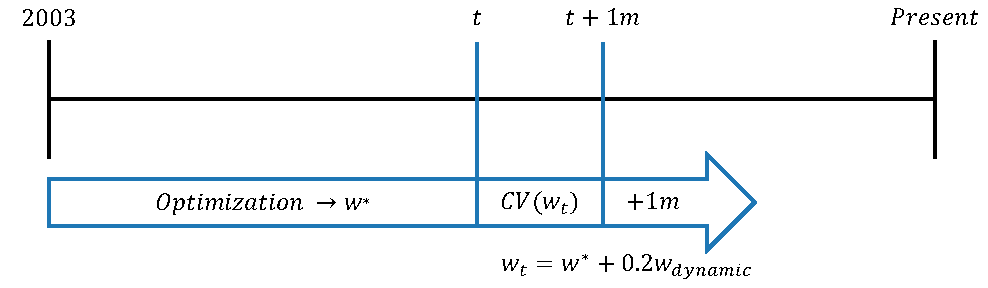
\includegraphics[width=\textwidth]{images/backtest_timeline.pdf}
    \end{center}
    \caption{\textbf{Iterative model performance validation methodology.}}
    \label{fig:backtest_timeline}
\end{figure}

The static threshold parameter $w^*$ itself is initially identified by evaluating a set of candidate values within the range $[0.6, 1.0]$ using incremental steps of $0.005$. For each threshold candidate, historical out-of-sample performance is evaluated to determine the combination yielding the highest product of market participation and active return. The threshold that maximizes this combined metric is chosen as the static threshold $w^*$.

This chapter established a comprehensive methodological framework for analyzing new issue premium in European investment-grade corporate bonds, progressing from data preprocessing through feature selection to model optimization and validation. The XGBoost-based approach, enhanced by ternary classification and hybrid threshold calibration, effectively captures complex relationships between bond characteristics and short-term performance. The resulting framework provides portfolio managers with a quantitative tool for systematic new issue evaluation, representing a significant advancement over traditional qualitative approaches and establishing the foundation for subsequent feature analysis and performance evaluation.